\cotefile{11}
\scanpage{3}
% e01: top, lines 1–2
$\mathcal V$ catégorie (\unsure{Objts} $X,Y,\ldots$) avec produits de deux objets
(\unsure{et} un objet final)

% e02: lines 3–5, with additions and cancellation
$A:\quad X\longrightarrow A(X)$ foncteur cov. de $\mathcal V$ dans la catégorie
\inserted{$C$} des Algèbres \inserted{gr.}, bivariant, satisfaisant une condition d'échange
\inserted{\unsure{entre les} $f^*$ et $f_*$} \deleted{\unsure{condition}}
(\unsure{dont le besoin sera vu dans la suite|dont le besoin est vu dès le suivant}\ldots).

% e03: lines 6–7
On va définir une nouvelle catégorie, notée $\mathcal V^A$, et
deux foncteurs $\varphi,\psi$
\diagram{\begin{tikzcd}[column sep=large,row sep=large]
\mathcal V \arrow[r,"\varphi"] \arrow[dr,"A"'] & \mathcal V^A \arrow[r,"\psi"] & k\text{-mod gr.} \\
& C \arrow[ur,"\omega"'] &
\end{tikzcd}}
\margin{$\omega$ oubli de \unsure{la} structure d'Algèbres,}
rendant le carré commutatif. De plus,
le foncteur $\varphi$ induit une bijection (en fait,
une identité) sur les ens. d'objets on \deleted{\unsure{identifie}}
\[
\operatorname{Ob}\mathcal V^A=\operatorname{Ob}\mathcal V
\]

% e04: middle
On pose
\[
\operatorname{Hom}_{\mathcal V^A}(X,Y)=A(X\times Y)
\]
On définit le produit de composition ainsi
\[
\begin{aligned}
\operatorname{Hom}_{\mathcal V^A}(X,Y)\times\operatorname{Hom}_{\mathcal V^A}(Y,Z)&\longrightarrow\operatorname{Hom}_{\mathcal V^A}(X,Z)\\
(u,v)&\longmapsto v\circ u
\end{aligned}
\]
\[
A(X\times Y)\times A(Y\times Z)\longrightarrow A(X\times Z)
\]
\diagram{\begin{tikzcd}[column sep=small]
& X\times Y\times Z \arrow[dl,"p_{12}"'] \arrow[d,no head,"p_{13}"] \arrow[dr,"p_{23}"] &\\
X\times Y & X\times Z & Y\times Z
\end{tikzcd}}
\[
\boxed{v\circ u=p_{31*}\bigl(p_{32}^*(\unsure{v})\,p_{21}^*(u)\bigr).}
\]
\mspage{2}
\scanpage{4}
% Reused typescript is upside down in the supplied scan; text order follows its reading orientation.
\mspage{3}
\begin{center}-3.2-\end{center}
\margin{\unsure{11}}
\[
\varpi:\operatorname{SL}(n+1)\longrightarrow\operatorname{PGL}(n)
\]
is the canonical isogeny, then with respect to the induced action of
$\operatorname{SL}(n+1)$, $o_{\mathbb P}(1)$ admits an $\operatorname{SL}(n+1)$-linearization. This follows
because $\operatorname{SL}(n+1)$ acts on the affine cone over $\mathbb P_n$, compatibly with
the given action of $\operatorname{PGL}(n)$ on $\mathbb P_n$. This linearization induces an
$\operatorname{SL}(n+1)$-linearization of $L_i$ for each $i$ (for the induced action of
$\operatorname{SL}(n+1)$), and therefore such a linearization for each product
\[
\bigotimes_{i=0}^{m}L_i^{\otimes r_i}.
\]
On the other hand, the $(n+1)^{\mathrm{st}}$ power of the $\operatorname{SL}(n+1)$-linearization of
$\underline{o}_{\mathbb P}(1)$, which is a linearization of $\underline{o}_{\mathbb P}(n+1)$, is induced, via $\varpi$,
from a $\operatorname{PGL}(n)$-linearization (cf. Chapter 1, §2). Therefore, the
$\operatorname{SL}(n+1)$-linearization of
\[
\bigotimes_{i=0}^{m}L_i^{r_i}
\]
is a $\operatorname{PGL}(n)$-linearization if $n+1$ divides each $r_i$.

In any case, by means of these linearizations we can define in-
variant sections of all the sheaves $\bigotimes_{i=0}^{m}L_i^{r_i}$. To construct such
invariant sections, let $X_0,\ldots,X_n$ be the canonical sections of $\underline{o}_{\mathbb P}(1)$
on $\mathbb P_n$. Let
\[
X_i^{(j)}=p_j^*(X_i)
\]
be the induced sections of $L_j$.

\uline{Definition} \uline{3.1}: For all sequences $\alpha_0,\ldots,\alpha_n$ of integers such that
\scanpage{5}
Associativité
\diagram{\begin{tikzcd}
X \arrow[r,no head,"u"] & Y \arrow[r,no head,"v"] & Z \arrow[r,no head,"w"] & T
\end{tikzcd}}
À prouver
\[
w(vu)=(wv)u
\]
\deleted{Le premier \unsure{mb} est égal à $\unsure{\gamma_*}$}

\diagram{\begin{tikzcd}[column sep=small,row sep=large]
&& X\times Y\times Z\times T \arrow[dl,"\alpha'"'] \arrow[dr,"\nu'"] &&\\
& X\times Y\times Z \arrow[dl,"\lambda"'] \arrow[d,"\mu"] \arrow[dr,"\nu",swap,"\deleted{\unsure{\mu}}"] && X\times Z\times T \arrow[dl,"\alpha",swap,"\deleted{\unsure{\lambda}}"] \arrow[d,"\gamma"] \arrow[dr,"\beta"] &\\
X\times Y & \unsure{Y|X}\times Z & X\times Z & X\times T & Z\times T
\end{tikzcd}}
\[
\begin{aligned}
w(vu)&\overset{\text{dfn}}=\gamma_*(\beta^*(w)\alpha^*(vu))\\
&\overset{\text{dfn de }vu}=\gamma_*\bigl(\beta^*(w)\alpha^*(\nu_*(\mu^*(v)\deleted{\unsure{,}}\lambda^*(u)))\bigr)\\
&=\gamma_*\Bigl(\beta^*(w)\nu'_*\bigl(\underbrace{\alpha'^*(\mu^*(v)\lambda^*(u))}_{\alpha'^*\mu^*(v)\,\alpha'^*\lambda^*(u)=p_{YZ}^*(v)\,p_{XY}^*(u)}\bigr)\Bigr)
\end{aligned}
\]
\inserted{car $\alpha^*\nu_*=\nu'_*\alpha'^*$ \fbox{\unsure{échange}}}
\margin{$\Vert$ form. de proj (att. signe!)}
\[
\deleted{\unsure{(-1)^{\overline w\,\overline{\nu'_*}}}}\;=\;\deleted{\unsure{\gamma_*}}\;
\nu'_*\left(\underbrace{\nu'^*\beta^*(w)}_{p_{ZT}^*(w)}\,p_{YZ}^*(v)\,p_{\unsure{YY|XY}}^*(u)\right)
\]
\[
=p_{XT*}\bigl(p_{ZT}^*(w)\,p_{YZ}^*(v)\,p_{XY}^*(u)\bigr)
\]

\diagram{\begin{tikzcd}[column sep=small,row sep=large]
&& X\times Y\times Z\times T \arrow[dl,"n'"'] \arrow[dr,"b'"] &&\\
& X\times Y\times T \arrow[dl,"a"'] \arrow[d,"c"] \arrow[dr,"b"] && Y\times Z\times T \arrow[dl,"n"'] \arrow[d,"l"] \arrow[dr,"m"] &\\
X\times Y & X\times T & Y\times T & Y\times Z & Z\times T
\end{tikzcd}}
\[
\begin{aligned}
(wv)u&=c_*(b^*(wv)\,a^*(u))\\
&=c_*\bigl(\underbrace{b^*(\unsure{n}_*\deleted{\unsure{v}}(m^*(w)l^*(v)))}_{n'_*\left(\underbrace{b'^*(m^*(w)l^*(v))}_{p_{ZT}^*(w)\,p_{YZ}^*(v)}\right)}\,a^*(u)\bigr)
\end{aligned}
\]
\margin{\fbox{formule d'échange}}
\[
=c_*\bigl(n'_*(p_{ZT}^*(w)\,p_{YZ}^*(v))\,a^*(u)\bigr)
\]
\margin{form. de pr. (att. signe!)}
\[
=\deleted{c_*}\,n'_*\bigl(p_{ZT}^*(w)\,p_{YZ}^*(v)\,
\deleted{\unsure{b}}\underbrace{\unsure{n'^*}\,a^*(u)}_{p_{XY}^*(u)}\bigr)
=p_{XT*}\bigl(p_{ZT}^*(w)\,p_{YZ}^*(v)\,\unsure{p_{XY}^*(u)}\bigr)
\]
\mspage{4}
\scanpage{6}
% Reused typescript, read after rotating the supplied image by 180 degrees.
\mspage{5}
\begin{center}-3.1-\end{center}
\uline{Chapter} \uline{3}. \uline{An} \uline{elementary} \uline{example}

The purpose of this chapter is to give, independently of the
forgoing theory, an exhaustive analysis of a single special class of
actions. This has two objectives: first of all, the concepts of
pre-stable and stable are worked out in a representative non-trivial
case. Secondly, by attacking this case directly, we can circumvent
the difficulties involved in extending the previous work to semi-simple
groups in characteristic $p$ (cf. Preface). And, in fact, we obtain the
result over the ring of integers, hence, \uline{a} \uline{fortiori}, over any field.
This will enable us later to construct the so-called arithmetic
schemes of moduli of abelian varieties.

We have no use for a ground field in this chapter: all the
schemes that we will consider will be of finite type over $\operatorname{Spec}(\mathbb Z)$.
$\mathbb A^n$, $\mathbb P_n$, and $\operatorname{PGL}(n)$ stand for the usual schemes \uline{over} $\uline{\mathbb Z}$. The
action we shall study is the canonical action:
\[
\sigma_m:\operatorname{PGL}(n)\times(\mathbb P_n)^{m+1}\longrightarrow(\mathbb P_n)^{m+1}
\]
\margin{$-$}
i.e. of projective transformations on sequences of points in projective
space.

\fbox{§1.} The first step is to obtain a large number of\inserted{\ }invariant affine
open subsets in $(\mathbb P_n)^{m+1}$. To this end, let $p_0,\ldots,p_m$ denote
the projections of $(\mathbb P_n)^{m+1}$ onto its $m+1$ factors. Let
$L_i=p_i^*(\underline{o}_{\mathbb P}(1))$. Now unfortunately, $\underline{o}_{\mathbb P}(1)$ admits no $\operatorname{PGL}(n)$-
linearization with respect to the action of $\operatorname{PGL}(n)$ on $\mathbb P_n$. However, if
\scanpage{7}
\uline{Unités} On définit
\[
\Delta_X\in\operatorname{Hom}_{\unsure{\mathcal V_c^A|\mathcal V^A}}(X,X)=A(X\times X)
\]
en considérant
\[
\delta_X:X-X\times X\qquad(\mathrm{diag})
\]
et définissant
\[
\Delta_X=\deleted{\unsure{\delta_{X*}A(\delta_X)}}A(\delta_X)_*(1_{A(X)})
\]
Prouvons que $\Delta_X$ est une unité \unsure{bilatère} pour la
composition : on a
\diagram{\begin{tikzcd}
X \arrow[r,no head,"\Delta_X"] & X \arrow[r,no head,"u"] & Y
\end{tikzcd}}
\[
u\circ\Delta_X=p_{31*}(p_{32}^*(u)\,p_{21}^*(\Delta_X))
\]
\diagram{\begin{tikzcd}[column sep=small]
&X\times X\times Y\arrow[dl,"p_{21}"']\arrow[d,no head]\arrow[dr,"p_{32}"]&\\
X\times X&X\times Y&X\times Y
\end{tikzcd}}
\[
\begin{aligned}
p_{21}^*(\Delta_X)&=\unsure{p_{21}^*|p'_{21}{}^*}(\delta_{X*}(1))
\overset{\text{\inserted{\fbox{échange}}}}=q_*(p^*(1))=q_*(1)\\
p_{32}^*(u)\,p_{21}^*(\Delta_X)&=p_{32}^*(u)\,q_*(1)=q_*(q^*(p_{32}^*(u)))
\end{aligned}
\]
\margin{form. de proj\quad Attention \uline{signe!}}
\diagram{\begin{tikzcd}[column sep=large,row sep=large]
X\times Y\arrow[r,"\delta_X\times\operatorname{id}_Y=q"]\arrow[d,"p"']&X\times X\times Y\arrow[d,no head,"p_{21}"]\\
X\arrow[r,no head,"\delta_X"]&X\times X
\end{tikzcd}}
\margin{\unsure{donc}\quad\fbox{\parbox{.35\linewidth}{signe $(-1)^{uX}$ ; pas de signe pour calculer \deleted{\unsure{que}} $\Delta_X\circ v=v$\quad $v:Y-X$}}}
\[
\deleted{\unsure{a}}\quad=q_*(u)\qquad\text{car }p_{32}q=\operatorname{id}_{X\times Y}
\]
donc
\[
u\circ\Delta_X=p_{31*}q_*(u)=u
\]
car \deleted{\unsure{q}} $p_{31}q=\operatorname{id}$

On procède de façon analogue pour $\Delta_X\circ u=u$.

\uline{Donc on trouve bien une catégorie $\mathcal V^A$}

[\uline{NB} Pour définir la composition on n'a eu besoin que
des $p_*,p^*$ pour projections $X\times Y\unsure{\rightleftarrows|\longrightarrow}X$ ; mais pour
\deleted{définir} \unsure{construire} les unités on a utilisé aussi $q_*,q^*$ pour
les imm. diagonales et leurs produits par un $Y$\ldots]
\mspage{6}
\scanpage{8}
% Reused typescript, reading orientation rotated 180 degrees.
\mspage{7}
\begin{center}-2.33-\end{center}
then:
\[
\begin{aligned}
\nu^{M\otimes f^*L^n}(x,\delta)&=\nu^{M\otimes f^*L^{n_0}}(x,\delta)+\nu^{f^*L^{n-n_0}}(x,\delta)\\
&=\nu^{M\otimes f^*L^{n_0}}(x,\delta)+(n-n_0)\nu^L(f(x),\delta).
\end{aligned}
\]
First of all, apply the first part of Proposition 2.17 to $\nu^{M\otimes f^*L^{n_0}}$.
We conclude that, for some $K$:
\[
\nu^{M\otimes f^*L^{n_0}}(x,\delta)\geq-K.
\]
Secondly, apply the second part of Proposition 2.17 to $\nu^L(y,\delta)$,
for $y\in S=Y^s_{(0)}(L)_k$. By\unsure{,,}Theorem 2.1, all these numbers are
strictly positive. Therefore, by the Proposition:
\[
\nu^L(y,\delta)\geq\epsilon>0
\]
for all $y\in Y^s_{(0)}(L)_k$, and $\delta\in\Delta(G)$. Therefore, if $n\geq\left[n_0+\frac K\epsilon+1\right]$,
we conclude
\[
\nu^{M\otimes f^*L^n}(x,\delta)>0
\]
whenever $x\in f^{-1}\{Y^s_{(0)}(L)\}_k$. Therefore, by Theorem 2.1, all such
$x$ are in $X^{\unsure{s}}_{(0)}(M\otimes f^*L^n)$. \uline{QED}
\scanpage{9}
De même, pour la \deleted{\unsure{définition}} vérification de l'associativité,
on n'a utilisé la formule de projection et la
formule d'échange que dans le cas
\diagram{\begin{tikzcd}[column sep=small,row sep=large]
&X\times Y\times P\arrow[dl]\arrow[dr]&\\
X\times P\arrow[dr,no head]&&Y\times P\arrow[dl,no head]\\
&P&
\end{tikzcd}}
mais pour vérifier que les $\unsure{\delta_X|\Delta_X}^{\unsure{s|?}}$ sont des
unités, on en avait besoin aussi dans un cas
\diagram{\begin{tikzcd}[column sep=small,row sep=large]
&X\times Y\arrow[dl]\arrow[dr,hook]&\\
X\arrow[dr,hook,"\mathrm{diag.}"']&&X\times X\times Y\arrow[dl,"\mathrm{proj}"]\\
&X\times X&
\end{tikzcd}}

\figure{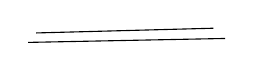
\begin{tikzpicture}\draw (0,0)--(2.5,.05);\draw (.1,.12)--(2.35,.18);\end{tikzpicture}}

Définissons le foncteur $\varphi$, en définissant pour
tt $X,Y\in\operatorname{Ob}\mathcal V$ une application
\[
\varphi_{X,Y}:\operatorname{Hom}_{\mathcal V}(X,Y)\longrightarrow
\operatorname{Hom}_{\mathcal V^A}(X,Y)=A(X\times Y)
\]
Soit donc $f:X\longrightarrow Y$ dans $\mathcal V$, on en définit
un hom graphe
\[
\Gamma_f=(\operatorname{id}_X,f):X-X\times Y
\]
d'où
\[
A(\Gamma_f)_*:A(X)\longrightarrow A(X\times Y)
\]
Posons alors
\[
\deleted{\unsure{A}}\quad\varphi_{X,Y}(f)=A(\Gamma_f)_*(1)
\]
\mspage{8}
\scanpage{10}
% Reused typescript; reading orientation rotated 180 degrees.
\mspage{9}
\begin{center}-2.32-\end{center}
$G$ on $X_1$ extending the given one on $X$, and there is an $M_1\in\operatorname{Pic}^G(X_1)$,
ample on $X_1$, which \inserted{extends} $M^N\otimes f^*L^{N_0N}$ for some $N$. (This $N$ may be taken
as the same $N$ as above). Then we have the diagram:
\diagram{\begin{tikzcd}[column sep=large,row sep=large]
X\arrow[r,"{(I_X,I_Y\circ f)}"]\arrow[d,"f"']&X_1\times Y_1\arrow[d,"p_2"]\\
Y\arrow[r,hook,"I_Y"']&Y_1
\end{tikzcd}}

Now if the result is proven when $X$ and $Y$ are proper, we can
apply it to $p_2:X_1\times Y_1\longrightarrow Y_1$, and the sheaves $M_1\otimes\underline{o}_{Y_1}$ on $X_1\times Y_1$
and $L_1$ on $Y_1$. Then
\[
\begin{aligned}
f^{-1}\{Y^s_{(0)}(L)\}&=f^{-1}\{I_Y^{-1}\{Y^s_{1(0)}(L_1)\}\}\\
&=(I_X,I_Y\circ f)^{-1}\{p_2^{-1}\{Y^s_{1(0)}(L_1)\}\}\\
&\subset (I_X,I_Y\circ f)^{-1}\{(X_1\times Y_1)^s_{(0)}(M_1\otimes L_1^n)\},\quad\text{if }n\geq n_0\\
&\subset X^s_{(0)}\left[(I_X,I_Y\circ f)^*(M_1\otimes L_1^n)\right]\quad\text{by Prop. 1},\\
&=X^s_{(0)}\left[M^N\otimes f^*L^{NN_0+Nn}\right]\\
&=X^s_{(0)}\left[M\otimes f^*L^{N_0+n}\right].
\end{aligned}
\]
Now, if $X$ and $Y$ are proper over $k$, we note again that
$M\otimes f^*L^n$ is ample on $X$ for $n\geq n_0$. Therefore, we can apply Theorem
2.1 to the computation of $X^s_{(0)}(M\otimes f^*L^n)$. But if $x\in X_k$, $\delta\in\Delta(G)$,
\scanpage{11}
Il faut prouver qu'on a bien un foncteur.

a) $\varphi_{X,X}(\operatorname{id}_X)=\Delta_X$. En effet,
\deleted{\unsure{ce qui est la définition}}\inserted{c'est la définition} de $\Delta_X$!

b) \diagram{\begin{tikzcd}X\arrow[r,no head,"f"]&Y\arrow[r,no head,"g"]&Z\end{tikzcd}}
\[
\varphi(g)\varphi(f)=\varphi(gf)
\]
Le premier mb est
\[
p_{31*}\left(\underbrace{p_{32}^*(\varphi(g))}_{\substack{p_{32}^*(\Gamma_{g*}(1))\\=\deleted{\unsure{\mu_*}}\lambda_*(\mu^*(1))=\lambda_*(1)}}\;
\underbrace{p_{21}^*(\varphi(f))}_{\substack{p_{21}^*\Gamma_{f*}(1)\\=\lambda'_*(\mu'^*(1))=\lambda'_*(1)}}\right)
\]
\diagram{\begin{tikzcd}[column sep=small,row sep=large]
&X\times Z\arrow[dl,"\mu'"']\arrow[dr,"\lambda'"]&&X\times Y\arrow[dl,"\lambda=\operatorname{id}_X\times\Gamma_g"']\arrow[dr,"\mu"]&\\
X\arrow[dr,"\Gamma_f"']&&X\times Y\times Z\arrow[dl,"p_{21}"]\arrow[d,"p_{31}"]\arrow[dr,"p_{32}"']&&Y\arrow[dl,"\Gamma_g"]\\
&X\times Y&X\times Z&Y\times Z&
\end{tikzcd}}
\[
\varphi(g)\varphi(f)=p_{31*}(\unsure{\lambda^*_*|\lambda_*}(1)\,\lambda'_*(1))
\]
Mais
\[
\lambda_*(1)\lambda'_*(1)=\lambda_*\left(\underbrace{\lambda^*(\lambda'_*(1))}_{\Gamma_{f*}(\Gamma_{gf}^*(1))=\Gamma_{f*}(1)}\right)
\qquad\fbox{\text{(form. proj)}}
\]
\diagram{\begin{tikzcd}[column sep=small,row sep=large]
&&X\arrow[dl,"\Gamma_{gf}"']\arrow[dr,"\Gamma_f"]&&\\
&X\times Z\arrow[dl,"\mu'=p_X"']\arrow[dr,"\lambda'=\unsure{\Gamma_f}\times Z"]&\text{(cartésien)}&X\times Y\arrow[dl,"\lambda=\operatorname{id}_X\times\Gamma_g"']\arrow[dr,"\mu=p_Y"]&\\
X\arrow[dr,"\Gamma_f"']&&X\times Y\times Z\arrow[dl,"p_{21}"]\arrow[d,"p_{31}"]\arrow[dr,"p_{32}"']&&Y\arrow[dl,"\Gamma_g"]\\
&X\times Y&X\times Z&Y\times Z&
\end{tikzcd}}
\[
=\lambda_*\Gamma_{f*}(1)=\nu_*(1)
\]
où $\nu:X-X\times Y\times Z$ est donné
par $\nu(x)=(x,f(x),gf(x))$.
\diagram{\begin{tikzcd}[column sep=small,row sep=small]
x\arrow[r,mapsto]&(x,gf(x))&(x,f(x),gf(x))\arrow[l,mapsto]\\
x\arrow[r,no head]&(x,f(x))\arrow[r,mapsto]&(x,f(x),gf(x))
\end{tikzcd}}
\margin{\deleted{\unsure{f(x)}} $(x,f(x),z)$\quad $(x,y,g(y))$\quad $(x,f(x),gf(x))$}
D'où
\[
\varphi(g)\varphi(f)=p_{31*}(\nu_*(1))=\Gamma_{gf*}(1)=\varphi(gf)\qquad\mathrm{OK}.
\]

\figure{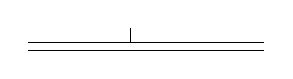
\begin{tikzpicture}\draw (0,0)--(3,0);\draw (0,-.10)--(3,-.10);\draw (1.3,0)--(1.3,.18);\end{tikzpicture}}

Définissons le foncteur $\psi$, \inserted{avec $\psi(X)=A(X)$,} i.e. pour
$u\in\operatorname{Hom}_{\mathcal V^A}(X,Y)=A(X\times Y)$, et $x\in A(X)$, définissons $u(x)\in A(Y)$
par formule \deleted{\unsure{u(x)}}
\[
u(x)=p_{2*}(u\,p_1^*(\unsure{x|u}))
\]
Prouvons que l'on a bien une \uline{loi fonctorielle}.
\mspage{10}
\scanpage{12}
% Reused typescript; reading orientation rotated 180 degrees.
\mspage{11}
\begin{center}-2.31-\end{center}
minimized is invariant under the transformation $z\longrightarrow\alpha z$, $\alpha>0$,
and the set of rays in $\unsure{\Gamma|\Pi}^{\mathbb R}(T)$ is \uline{compact}. We must check that this
``inf'' is actually attained by a rational point $z$. But each linear
functional $\ell_{\unsure{j|i}}$ is rational, and the inner product $\langle x,y\rangle$ on $\unsure{\Gamma|\Pi}^{\mathbb R}(T)$
is rational: then it is an exercise in elementary calculus to check
that this is so. \uline{QED}

An application of this is:

\uline{Proposition} \uline{2.18}: Let $G$ be a reductive group acting on algebraic
schemes $X$ and $Y$. Let $f:X\longrightarrow Y$ be a $G$-linear morphism, let
$L\in\operatorname{Pic}^G(Y)$ and $M\in\operatorname{Pic}^G(X)$. Then if $M$ is relatively ample for $f$
and $L$ is ample on $Y$, there is an $n_0$ such that:
\[
n\geq n_0\Longrightarrow X^s_{(0)}(M\otimes f^*L^n)\supset f^{-1}\{Y^s_{(0)}(L)\}.
\]

\uline{Proof}: We shall first reduce this Proposition to the case where
$X$ and $Y$ are proper over $k$. First of all, there is an open immer-
sion $I_Y:Y\subset Y_1$, where $Y_1$ is proper over $k$, and there is an
action of $G$ on $Y_1$ extending the given one of $G$ on $Y$, and there
is an $L_1\in\operatorname{Pic}^G(Y_1)$, ample on $Y_1$ which extends $L^N$ for some $N$,
such that:
\[
Y^s_{(0)}(L)=I_Y^{-1}\{Y^s_{1(0)}(L_1)\}
\]
(cf. Proposition 1.8). Secondly, for some $N_0$, $M\otimes f^*L^{N_0}$ is ample
on $X$ by EGA2, \unsure{4.6:13|4.6.13}, (ii). Then there is also an open immersion
$I_X:X\subset X_1$, where $X_1$ is proper over $k$, and there is an action of
\scanpage{13}
a) Si $X=Y$, prouvons que $\Delta_X(x)=x$. On a
\[
\begin{aligned}
\Delta_X(x)&=p_{2*}(\Delta_X\,p_1^*(x))
=p_{2*}\bigl(\underbrace{\delta_*(1)\,p_1^*(x)}_{\delta_*(1\cdot\underbrace{\delta^*p_1^*(x)}_x)}\bigr)\\
&=p_{2*}\delta_*(x)=x\qquad\mathrm{OK}.
\end{aligned}
\]
\margin{form. de proj}
\diagram{\begin{tikzcd}[column sep=small]
&X\arrow[d,"\delta"']&\\
&X\times X\arrow[dl,"p_1"']\arrow[dr,no head,"p_2"]&\\
X&&X
\end{tikzcd}}

b) Prouvons $v(u(x))=(v\circ u)(x)$.
\diagram{\begin{tikzcd}X\arrow[r,"u"]&Y\arrow[r,"v"]&Z\end{tikzcd}}
\diagram{\begin{tikzcd}[column sep=small,row sep=large]
&&X\times Y\times Z\arrow[dl,"\lambda=p_{XY}"']\arrow[dr,"\mu=p_{YZ}"]&&\\
&X\times Y\arrow[dl,"p_1"']\arrow[dr,"p_2"]&&Y\times Z\arrow[dl,"q_1"']\arrow[dr,"q_2"]&\\
X&&Y&&Z
\end{tikzcd}}
\[
\begin{aligned}
v(u(x))&=\deleted{\unsure{q_{1*}}}\;q_{2*}(v\,q_1^*u(x))\\
&=q_{2*}\Bigl(v\,\underbrace{q_1^*\bigl(p_{2*}(u\,p_1^*(x))\bigr)}_{\substack{\mu_*(\lambda^*(u\,p_1^*(x)))\\=\mu_*(\lambda^*(u)\,p_X^*(x))}}\Bigr)
\end{aligned}
\]
\margin{\fbox{échange}}
\deleted{$\unsure{=}$}\quad\deleted{$\unsure{=}$}
\[
=q_{2*}\bigl(\mu_*(\mu^*(v)\,\lambda^*(u)\,p_X^*(x))\bigr)
\]
\margin{proj, attention signe}
\[
=p_{Z*}(p_{YZ}^*(v)\,p_{XY}^*(u)\,p_X^*(x))
\]
On a d'autre part
\diagram{\begin{tikzcd}[column sep=small,row sep=large]
&X\times Y\times Z\arrow[dl,"p_{XY}"']\arrow[d,"p_{YZ}"]\arrow[dr,"p_{XZ}"]&\\
X\times Y&\unsure{YZ|Y\times Z}&X\times Z\arrow[dll,"r_1"']\arrow[d,"r_2"]\\
X&&Z
\end{tikzcd}}
\[
\begin{aligned}
(v\circ u)(x)&=r_{2*}((v\circ u)\,r_1^*(x))\\
&=r_{2*}\Bigl(\underbrace{p_{XZ*}(p_{YZ}^*(v)\,p_{XY}^*(u))\,r_1^*(x)}_{p_{XZ*}(p_{YZ}^*(v)\,p_{XY}^*(u)\,\underbrace{p_{XZ}^*r_1^*(x)}_{p_X^*(x)})}\Bigr)\\
&=p_{Z*}(p_{YZ}^*(v)\,p_{\unsure{XZ|XY}}^*(u)\,p_X^*(x))
\end{aligned}
\]
OK.
\mspage{12}
\scanpage{14}
% Reused typescript; reading orientation rotated 180 degrees.
\mspage{13}
\begin{center}-2.30-\end{center}
\uline{Proof}: Let $T\subset G$ be a maximal torus. Let $\langle x,y\rangle$ be the form
on $\unsure{\Gamma|\Pi}^{\mathbb R}(T)$ which defines the norm $\Vert\lambda\Vert$. Let $\ell_1,\ldots,\ell_n$ be the
linear functionals on $\unsure{\Gamma|\Pi}^{\mathbb R}(T)$ given by Proposition 2.14. For any
$x\in X_k$, let $I(x)$ be the subset $\{1,\ldots,n\}$ given by Proposition 2.14.
To estimate $\nu^L(x,\delta)$, say $\delta=\Delta(\lambda)$. There is always some $\gamma\in G_k$
such that $\gamma\circ\lambda\circ\gamma^{-1}$ is a 1-PS of $T$. Then:
\[
\begin{aligned}
\nu^L(x,\delta)&=\frac{\mu^L(x,\lambda)}{\Vert\lambda\Vert}\\
&=\frac{\mu^L(\sigma(\gamma,x),\gamma\circ\lambda\circ\gamma^{-1})}{\Vert\uline{\gamma\circ\lambda\circ\gamma^{-1}}\Vert}\\
&=\max\left\{\frac{\ell_i(\gamma\circ\lambda\circ\gamma^{-1})}{\sqrt{\langle\gamma\circ\lambda\circ\gamma^{-1},\gamma\circ\lambda\circ\gamma^{-1}\rangle}}\;\middle|\;i\in I(\sigma(\gamma,x))\right\}
\end{aligned}
\]
But, for each $i$, $|\ell_i(z)|/\sqrt{\langle z,z\rangle}$ is bounded when $z$ varies
over all non-zero points of $\unsure{\Gamma|\Pi}^{\mathbb R}(T)$. Therefore $\nu^L(x,\delta)$ is bounded
when $x$ and $\delta$ vary arbitrarily. Now suppose for $x\in S\subset X_k$, we seek
to minimize $\nu^L(x,\delta)$. According to the above,
\[
\inf_{\substack{\delta\in\Delta(G)\\x\in S}}\nu^L(x,\delta)
=\inf_{\substack{\gamma\in G_k\\x\in S}}\left[\inf_{z\in\unsure{\Gamma|\Pi}^{\mathbb Q}(T)}\left[\max_{i\in I(\sigma(\gamma,x))}\frac{\ell_i(z)}{\sqrt{\langle z,z\rangle}}\right]\right]
\]
But the first ``inf'' is essentially a minimum over the finite set of
subsets $I\subset\{1,\ldots,n\}$ which occur as subsets $I(\sigma(\gamma,x))$. Therefore,
this ``inf'' will always be attained for some $x$ and $\gamma$. As for the
inner ``inf'', if we replace the variable \inserted{by} $z\in\unsure{\Gamma|\Pi}^{\mathbb R}(T)$, then the ``inf''
will certainly be attained for some $z$ - for the expression to be
\scanpage{15}
Commutativité du carré de foncteurs.
Il suffit de le voir sur les flèches, donc : \unsure{prouvons}
pour $f:X\longrightarrow Y$ dans $\mathcal V$, et $x\in A(X)$
\[
f_*(x)=\varphi(f)(x)
\]
Or on a
\diagram{\begin{tikzcd}[column sep=small]
&X\arrow[d,no head,"\Gamma_f"]&\\
&X\times Y\arrow[dl,"p_1"']\arrow[dr,no head,"p_2"]&\\
X&&Y
\end{tikzcd}}
\[
\begin{aligned}
\varphi(f)(x)&=p_{2*}(\varphi(f)\,p_1^*(x))
=p_{2*}\bigl(\underbrace{\Gamma_{f*}(1)\,p_1^*(x)}_{\Gamma_{f*}(\underbrace{\Gamma_f^*p_1^*(x)}_x)}\bigr)\\
&=p_{2*}\Gamma_{f*}(x)=x\qquad\mathrm{OK}.
\end{aligned}
\]

\deleted{\uline{\unsure{Question:}}}\inserted{Remarque}
Comment interpréter le foncteur
contravariant $\mathcal V^\circ-k\text{-mod gr}$ défini par $A$,
en composant $A$ et le foncteur $\omega^*:C^\circ\longrightarrow k\text{-mod gr}$
(associant à $(f_*,\unsure{f^*})$ l'application $f^*$)? En d'autres
termes, comment interpréter $A(f)^*:A(Y)-A(X)$,
si $f:Y\longrightarrow X$? On devine que c'est défini
par $\varphi(f)^*\in\operatorname{Hom}_{\mathcal V^A}(Y,X)=A(Y\times X)$, déduit
de $\varphi(f)\in\unsure{H|A}(X\times Y)$ par l'isom can. qu'on
devine. Vérification comme dessus.

On définit un anti-foncteur canonique
\[
\unsure{s}:\unsure{\mathcal V^{A\circ}}-\unsure{\mathcal V^{A\circ}},
\]
induisant l'identité sur les objets, par
\[
u\longmapsto{}^su:\operatorname{Hom}_{\mathcal V^A}(X,Y)=A(X\times Y)-\operatorname{Hom}_{\mathcal V^A}(Y,X)=A(Y\times X)
\]
\margin{vérifier que c'est \uline{\unsure{multiplicatif}!}}
\mspage{14}
\scanpage{16}
% Reused typescript, rotated 180 degrees in the scan.
\figure{\begin{tikzpicture}\draw(0,0)--(.35,-.03);\draw(.65,-.06)--(.9,-.1);\end{tikzpicture}}
\begin{center}-2.29-\end{center}

\uline{Proof}: Immediate, since $\overline{\lambda_1\circ\lambda_2}=\bar\lambda_1+\bar\lambda_2$.

\uline{Corollary 2.16}: Let a reductive $G$ act on $X$, proper over $k$. Let $L\in\operatorname{Pic}^G(X)$ be ample, and let $x\in X_k$. Then $\{\delta\mid\nu^L(x,\delta)\leq0\}$ is semi-convex, and $\{\delta\mid\nu^L(x,\delta)<0\}$ is convex.

\uline{Proof}: Immediate.

It follows that from this Corollary and from Theorem 2.1, that if $\unsure{x}\in X_k$ is not \uline{semi-stable}, then we can associate to $x$ the convex set $C$ of $\delta\in\Delta(G)$ for which $\nu^L(x,\delta)<0$. Roughly speaking, we can say that a parabolic subgroup $P$ is ``responsible'' for this break-down of semi-stability if $C\cap\Delta_P(G)\neq\unsure{\phi|\varnothing}$. Since $C$ is convex, not too many parabolic subgroups $P$ are responsible; according to a conjecture of Tits, there is \inserted{even} a natural way to find one $P$ which is \uline{most} responsible, i.e.\ $P(\delta)$ for $\delta=$ the ``center'' of $C$ (cf.\ Preface).
Another consequence of Proposition 2.14 is:

\uline{Proposition 2.17}: Let a reductive $G$ act via $\sigma$ on $X$, proper over $k$. Let $L\in\operatorname{Pic}^G(X)$ be ample. Then there is a constant $K$ such that
\[
|\nu^L(x,\delta)|\leq K
\]
for all $x\in X_k$ and $\delta\in\Delta(G)$. Moreover, for every subset $S\unsure{\subset}X_k$, there is a $\delta_0\in\Delta(G)$ and $x_0\in S$ such that
\[
\nu^L(x_0,\delta_0)\leq\nu^L(x,\delta)^{\unsure{\circ|0}}
\]
for every other $\delta\in\Delta(G)$, $x\in S$.
\mspage{15}
\scanpage{17}
% Upper continuation and insertion.
\inserted{\unsure{provenant de}} l'isom canonique entre $X\times Y$ et $Y\times X$. Soit alors
\[
\varphi^*=s\varphi^\circ:\mathcal V^\circ\longrightarrow\mathcal V^A.
\]
on \unsure{constate} alors que le composé
\[
\psi\varphi^*=\psi(s\varphi^\circ)=(\psi s)\varphi^\circ:\mathcal V^\circ\longrightarrow k\text{-mod gr}
\]
est \deleted{\unsure{donc}} \uline{égal} à $\omega^*A^\circ:\mathcal V^\circ\longrightarrow k\text{-mod gr}$.
\margin{\uline{vérifier}}

\deleted{Ainsi, $\mathcal V^A$ \unsure{apparaît comme une espèce d'enveloppe}}

% Middle paragraph.
\uline{Car si $\mathcal V$ a un objet final $e$, et si de plus} $A(e)=k$ \inserted{[Sinon, on remplace $k$ par $A(e)$!]} Alors les $A(X)$ sont naturellement jaugés; si c'est des Alg. de Poincaré, il suffit alors de connaître \deleted{\unsure{les}} Alg. jaugées, $+$ les $f^*$ ($f:X-Y$ de $\mathcal V$) pour connaître $A$.

Soit
\[
\begin{aligned}
u&\in\operatorname{Hom}_{\mathcal V^A}(X,Y)=A(X\times Y)\\
su&\in\operatorname{Hom}_{\mathcal V^A}(Y,X)=A(Y\times X)
\end{aligned}
\]
donc $\tilde u:A(X)\longrightarrow A(Y)\qquad\widetilde{su}:A(Y)\longrightarrow A(X)$.

Montrons que \inserted{si $u$ central dans $A(X\times Y)$, alors} $\tilde u$ et $\widetilde{su}$ sont transposés l'un de l'autre, pour les formes $\unsure{k|\kappa}_{A(X)}$ et $\unsure{k|\kappa}_{A(Y)}$ sur $A(X)$, $A(Y)$, i.e.\ on a pour $x\in A(X)$, $y\in A(Y)$, $u\in A(X\times Y)$
\[
\unsure{k|\kappa}_Y\bigl(y\unsure{\tilde u_*(x)|u_*(x)}\bigr)=\unsure{k|\kappa}_X\bigl(\unsure{\tilde u^*(y)|u^*(y)}x\bigr)\qquad\text{i.e.}
\]
\[
g_*(y u_*(x))=f_*(u^*(y)x).\quad(\uuline{\text{Car $u$ central!}})\quad\text{En effet}
\]
\margin{$\unsure{g^*}$}
\diagram{\begin{tikzcd}
A(X)\arrow[r,shift left,"u_*"]\arrow[d,"\unsure{k|\kappa}_X"'] & A(Y)\arrow[l,shift left,"u^*"]\arrow[d,"\unsure{k|\kappa}_Y"]\\
k\arrow[r,phantom,"="]&k
\end{tikzcd}}
\diagram{\begin{tikzcd}
&X\times Y\arrow[dl,no head,"p_1"']\arrow[dr,no head,"p_2"]&\\
X\arrow[dr,no head,"f"']&&Y\arrow[dl,no head,"g"]\\
&e&
\end{tikzcd}}
\[
\begin{aligned}
g_*(y u_*(x))
&=\unsure{g_*}\bigl(y p_{2*}(u p_1^*(x))\bigr)
=g_*p_{2*}(p_2^*(y)u p_1^*(x))
=\unsure{k(p_2^*(y)u p_1^*(x))}\\
f_*(u^*(y)x)
&=f_*\bigl(p_{1*}(u p_2^*(y))x\bigr)
=f_*p_{1*}(u p_2^*(y)p_1^*(x))
=k(u p_2^*(y)p_1^*(x))\\
&\unsure{\geq|=}\ k(p_2^*(y)u p_1^*(x))
\end{aligned}
\]
\margin{$\boxed{\text{mod. signe!}}$}
\figure{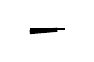
\begin{tikzpicture}\draw[line width=1.5pt] (0,0)--(.35,.03);\draw (0,.04)--(.45,.04);\end{tikzpicture}}
\mspage{16}
\scanpage{18}
% Reused typescript, rotated 180 degrees in the scan.
\begin{center}-2.28-\end{center}
\[
L^N=\phi^*(\underline{o}(1))
\]
Therefore:
\[
\mu^L(x,\lambda)=\frac1N\mu^{o(1)}(\phi x,\lambda).
\]
As in \S1, the action of $G$ on $\mathbb P_{n-1}$ is induced by a linear representation of $G$ in the affine cone $\mathbb A^n$ over $\mathbb P_{n-1}$. Suppose we choose coordinates in $\mathbb A^n$ so that the representation of $T$ is diagonalized: i.e.\ $\alpha\in T_k$ acts via the matrix $\{\chi_i(\alpha)\cdot\delta_{ij}\}$ for suitable characters $\chi_1,\ldots,\chi_n$ of $T$. Let $\chi_i$ induce the linear functional $\bar\chi_i$ on $\unsure{\Gamma|\Pi}^{\mathbb R}(T)$, and as usual let a 1-PS $\lambda$ of $T$ induce the point $\bar\lambda\in\unsure{\Gamma|\Pi}^{\mathbb R}(T)$. Then if $(\phi x_1^*,\ldots,\phi x_n^*)$ are coordinates of a homogeneous point lying over $\phi x$, Proposition 2.3 asserts:
\[
\mu^{o(1)}(\phi x,\lambda)=\max\{-\bar\chi_i(\bar\lambda)\mid i\text{ such that }\phi x_i^*\neq0\}.
\]
We conclude:

\uline{Proposition 2.14}: Let a reductive $G$ act on $X$, proper over $k$. Let $T\subset G$ be a maximal torus, and let $L\in\operatorname{Pic}^G(X)$ be ample. Then there is a finite set of linear functionals $\ell_1,\ldots,\ell_n$ on $\unsure{\Gamma|\Pi}^{\mathbb R}(T)$ which are rational on $\unsure{\Gamma|\Pi}^{\mathbb Q}(T)$ with the following property:

\begin{quote}
for every $x\in X_k$, there is a subset $I\subset\{1,\ldots,n\}$ such that $\mu^L(x,\lambda)=\max\{\ell_i(\bar\lambda)\mid i\in I\}$ for all 1-PS's $\lambda$ of $T$.
\end{quote}

\uline{Corollary 2.15}: If $\lambda_1,\lambda_2$ are 1-PS's of $T$ and $x\in X_k$, then
\[
\mu^L(x,\lambda_1\circ\lambda_2)\leq\mu^L(x,\lambda_1)+\mu^L(x,\lambda_2)
\]
\mspage{17}
\scanpage{19}
\uline{Remarque} On n'a jamais, dans les calculs précédents, utilisé la structure additive des $A(X)$, seulement leur structure de monoïde. Donc il y a lieu de formuler la théorie des correspondances en prenant \deleted{\unsure{des}} $X\longrightarrow A(X)$ \deleted{qui sont des} \inserted{foncteurs dans les} ``monoïdes bivariants'' \ldots.

\deleted{Il faudrait être \deleted{\unsure{prudent}} \inserted{\unsure{rigoureux}} pour les signes, dans le cas de monoïdes non commutatifs, en prenant des monoïdes gradués [\unsure{les degrés en} \unsure{anneaux anticommutatifs}}

Ce point de vue cependant ne semble pas très commode dans le cas ou les 2 formules de projections \inserted{(gauche et droite)} ne sont pas valables l'une et l'autre, et qu'il faut introduire des signes. Il faudrait alors remplacer les monoïdes par des ``monoïdes jaugés'' $(A^i)_{i\in\mathbb Z}$, loi de composition $A^i\times\unsure{A^j}-A^{i+j}$ (NB: L'ensemble somme des $A^i$ \deleted{\unsure{est}} muni d'une structure de monoïde) et \deleted{\unsure{automorphismes involutifs d'ordre}} \inserted{applications bijectives} $\sigma^i:A^i-A^i$ satisfaisant $\unsure{\sigma^{i\,2}|(\sigma^i)^2}=\operatorname{id}$, $\sigma^i=\operatorname{id}$ si $i$ pair, \deleted{\unsure{pour}} enfin chaque $A^*$ muni d'un \uline{degré} \inserted{$d(A^*)$} qui permet d'imposer le degré des $\unsure{f_*|f_s}$ des $(\unsure{f_*,f^*|f=(f^i)}):A^*\unsure{\longrightarrow|-}B^*$ comme $\deleted{\unsure{f|d}}d(B^*)-d(A^*)$. On peut alors \unsure{indiquer} comment les \uline{signes} doivent être calculés dans la formule de projection gauche (si on veut que la droite soit \unsure{valable}).
\mspage{18}
\scanpage{20}
% Reused typescript, rotated 180 degrees in the scan.
\begin{center}-2.26-\end{center}
\uline{Proof}: $T_1$ and $T_2$ are both maximal tori in $P(\delta_1)\cap P(\delta_2)$ by lemma 2.9. Therefore they are conjugate in $P(\delta_1)\cap P(\delta_2)$. \uline{QED}

Now suppose $\delta_1$, $\delta_2$ are, in fact, in $\Delta(T_1)\cap\Delta(T_2)$: we must show that the lines joining them in $\Delta(T_1)$ and in $\Delta(T_2)$ are the same. Let $T_1=\gamma^{-1}\cdot T_2\cdot\gamma$ and suppose $\lambda_1,\lambda_2$ are 1-PS's of $T_2$ representing $\delta_1,\delta_2$, respectively. Then $\gamma^{-1}\cdot\lambda_1\cdot\gamma$, $\gamma^{-1}\cdot\lambda_2\cdot\gamma$ are 1-PS's of $T_1$ representing $\delta_1,\delta_2$ respectively. Therefore, we must show that the sets of points
\[
\{\Delta(\lambda_1^{n_1}\cdot\lambda_2^{n_2})\}\quad\text{and}\quad
\{\Delta((\gamma^{-1}\lambda_1\gamma)^{n_1}\cdot(\gamma^{-1}\cdot\lambda_2\cdot\gamma)^{n_2})\}
\]
are the same. But this is clear provided that $\Delta(\lambda_1^{n_1}\cdot\lambda_2^{n_2})=\Delta(\gamma^{-1}\lambda_1^{n_1}\cdot\lambda_2^{n_2}\gamma)$; hence it follows it $P(\lambda_1)\cap P(\lambda_2)\subset P(\lambda_1^{n_1}\cdot\lambda_2^{n_2})$ - so that $\gamma\in P(\lambda_1^{n_1}\cdot\lambda_2^{n_2})$.

Therefore, we are reduced to proving that if $\lambda_1$, $\lambda_2$ are 1-PS's of $G$ which centralize each other, then
\[
(**)\qquad P(\lambda_1\cdot\lambda_2)\supset P(\lambda_1)\cap P(\lambda_2)
\]
To prove this, it is convenient to represent $G$ in $\operatorname{GL}(n)$ by some closed immersion $\phi:G\longrightarrow\operatorname{GL}(n)$. Then, exactly as in the proof of Proposition 2.6, we have reduced the proof of $(**)$ to the case $G=\operatorname{GL}(n)$. In this case, we can simultaneously diagonalize two commuting 1-PS's: say $\lambda_1(\alpha)$ is the matrix $\{\alpha^{r_i}\cdot\delta_{ij}\}$, and $\lambda_2(\alpha)$ is the matrix $\{\alpha^{s_i}\cdot\delta_{ij}\}$, for $\alpha\in(\mathbb G_m)_k$. Then, as in Proposition 2.6,
\mspage{19}
\scanpage{21}
Pour tout $X\in\mathcal V$, les $A'(X)\subset A(X)$, \inserted{avec $1_{A(X)}\in A'(X)$, stable par \unsure{``signe''}} conditions équiv.

$1^\circ)$ Les $A'(X)$ stables par images inverses, images directes pour \textcircled{tout} morphisme de $\mathcal V$, et par produits [ou encore, par produits $\boxtimes$].

$2^\circ)$ \deleted{Si} a) $u\in A'(X\times Y)$, $x\in A'(X)$, alors $u_*(x)\in A'(Y)$.

b) Si $x\in A'(X)$, $y\in A'(Y)$, alors $x\boxtimes y\in A'(X\times Y)$.

c) Pour \textcircled{tout} morphisme $X-Y$ [il suffit de prendre les\hspace{1cm}] le graphe $\gamma_f=\Gamma_{f*}(1)\in A(X\times Y)$ est dans $A'(X\times Y)$.
\margin{\figure{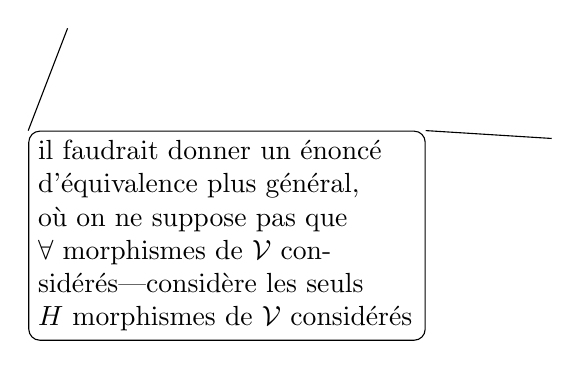
\begin{tikzpicture}\node[draw,rounded corners,text width=4.8cm] (m) {il faudrait donner un énoncé d'équivalence plus général, où on \unsure{ne suppose pas que $\uline{\forall}$ morphismes de $\mathcal V$ considérés|considère les seuls $H$ morphismes de $\mathcal V$ considérés}};\draw (m.north west)--++(.5,1.3);\draw (m.north east)--++(1.6,-.1);\end{tikzpicture}}}

\deleted{\uline{NB} Ces $A'$ correspondent aux ss-catégories (\unsure{pas pleines}) de $\mathcal V^A$ ayant \unsure{mêmes objets} que $\mathcal V^A$,}
\margin{\uline{NB} Si $\mathcal V$ a un objet final, les $A'$ correspondent exactement aux ss-catégories de $\unsure{\mathcal V_A|\mathcal V^A}$ qui ont \unsure{même ens.|ts ces} \deleted{\unsure{anneaux, et}} d'objets que $A$, stables par $\boxtimes$ de flèches, et contenant les \deleted{\unsure{projections des produits}} morphismes de $\mathcal V$ et leurs ${}^s\Gamma_f$ (il suffit ${}^s\unsure{\delta_X|\gamma_X}$).}

\uline{Dém} $1^\circ)\Longrightarrow2^\circ)$

$1^\circ$ forme \unsure{croisée} [avec $\boxtimes$] implique forme \unsure{non croisée}, car
\[
x\odot y=\delta^*(x\boxtimes y)\qquad[x,y\in A(X),\quad\delta=\operatorname{diag}_X:X-X\times X]
\]
\margin{image inverse par $\delta$}

$1^\circ$ forme \unsure{non croisée} implique forme \unsure{croisée}, car
\[
x\boxtimes y=p_1^*(x)p_2^*(y).
\]
\margin{$\boxed{\text{image inverse par }\unsure{p_i|\operatorname{pr}}}$}

a) car
\[
u_*(x)=p_{2*}(u p_1^*(x)).
\]
\margin{[De même pour $u^*(y)\in A'(X)$ si $y\in A'(Y)$]}
\margin{$\boxed{\text{image directe, inverse par }\unsure{p_i|\operatorname{pr}}}$}

b) clair

c) clair, car $1_X\in A'(X)$ par hyp.
\margin{$\boxed{\text{image directe de 1 par un graphe}}$}
\margin{$+\ \textcircled{\unsure{produit}}$}

$2^\circ)\Longrightarrow1^\circ)$. Stabilité par image \deleted{\unsure{directe}} directe: car $f_*(x)=\deleted{\unsure{\xi_f}}\gamma_f(x)$, on applique a) et c).

Stabilité par image \deleted{directe} \inserted{inverse}: car $f^*(y)=({}^{\unsure{s|t}}\gamma_f)_*(y)$, et comme $\gamma_f\in A'(X\times Y)$, on a ${}^{\unsure{s|t}}\gamma_f\in A'(Y\times X)$ (stabilité par isom),

Stabilité par $\boxtimes$ claire.
\mspage{20}
\scanpage{22}
% Reused typescript, upright in the scan.
\begin{center}-2.24-\end{center}
of the terminology ``flag complex''.

A second direction in which we can make explicit this structure on $\Delta(G)$ is to show that the skeletons are pasted together in a sufficiently nice way so that various constructions which can be carried out in each skeleton, can also be carried out in $\Delta(G)$. The principal one we have in mind is drawing a great circle through two points. One approach to this is to complete the complex $\Delta(G)$ with respect to the metric $\rho$ mentioned above: then Tits has shown that the geodesic segments on this completion are precisely the segments of great circles of length $\leq\pi$, on the true spheres obtained by completing the skeletons $\Delta(T)$. Since we are avoiding this metric, we define these lines, and other auxiliary concepts, directly:

\uline{Definition 2.8}: A pair of points $\delta_1,\delta_2\in\Delta(T)$ is \uline{antipodal} if there is a 1-PS $\lambda$ of $G$ such that $\delta_1=\Delta(\lambda)$ and $\delta_2=\Delta(\lambda^{-1})$.

If $G$ is a torus, then every point of $\Delta(G)$ has a unique antipodal point, i.e.\ its antipodal on the sphere is the usual sense. More general, if $\delta_1$ is in the skeleton $\Delta(T)$ of $\Delta(G)$, for some maximal torus $T$, then the antipodal $\delta_2$ of $\delta_1$ as a point of $\Delta(T)$, is one of its antipodal points in $\Delta(G)$. In fact, these are the only points antipodal to $\delta_1$:

\uline{lemma 2.12}: If $\delta_1,\delta_2$ are two points in the skeleton $\Delta(T)$ of $\Delta(G)$, for some maximal torus $T$, then $\delta_1$ and $\delta_2$ are antipodal as points of $\Delta(G)$ if and only if they are antipodal as points of the sphere $\Delta(T)$.
\mspage{21}
\scanpage{23}
\deleted{\unsure{Intersections Sommes}}

Sous-Anneaux bivariants sur $\mathcal V$. [\unsure{tels que|cela fait}: \unsure{on compte} les form. de proj. et d'échange]
Intersection de tels est idem; d'où notion de \unsure{foncteur} ``stable'' \uuline{engendré}. Soit $A_{\mathrm{sp}}\deleted{\unsure{\in}}\subset A$ le plus petit ss-foncteur stable engendré.

\uline{NB} $A_{\mathrm{sp}}(X)$ contient les $f_*(1_Y)$ pour $f:Y-X$ dans $\mathcal V$. Dans beaucoup de cas importants, il est $=$ identique à \unsure{l'ens} des $f_*(1_Y)$ pour tous les $f:Y-X$ de $\operatorname{Ob}(\mathcal V_{/X})$. Cela marche p.ex.\ si $\mathcal V$ la catégorie des schémas projectifs lisses \unsure{équidim} sur $k$ alg. clos, dans les cas envisagés plus haut, du moins si on admet la résolution des \uline{singularités}.

\margin{$A'\subset A$ donné, \uline{stable}}
Une application $A(X_{\unsure{1}})\times\cdots\times A(X_n)\longrightarrow A(X)$ est dite \uline{de type} $A'$ si elle est de la forme
\[
x_1,\ldots,x_n\longmapsto u(x_1\boxtimes\cdots\boxtimes x_n)
\]
avec $u\in A'(X_1\times\cdots\times X_n\times X)$. En \deleted{\unsure{un cas}} particulier, ceci est défini si $n=1$.
Composer une \inserted{telle} application $\varphi$ avec une application $\psi:A(X)-A(X')$ qui est de type $A'$, on trouve une application qui est de type $A'$.

\deleted{\unsure{De}} \deleted{Plus gén.} \deleted{De même,} \inserted{Plus gén.} si on compose des applications
\deleted{Donnons nous des \unsure{fonctions} $(\unsure{\varphi_i})_{i\in I}$}
\[
\begin{aligned}
\varphi(x_1,\ldots,x_n)&:A(X_1)\times\cdots\times A(X_n)-A(X)\\
\psi(y_1,\ldots,y_m)&:A(Y_1)\cdots\times A(Y_m)-A(Y)
\end{aligned}
\]
\deleted{\unsure{-}} avec $\chi:A(X)\times A(Y)\longrightarrow A(Z)$
\mspage{22}
\scanpage{24}
\begin{center}-2.23-\end{center}
Therefore, in view of lemma 2.9, $\Delta(G)$ can be viewed as the result of pasting together spheres, one for each $T\subset G$, with sufficient identifications so that any two points are both on at least one sphere. The subsets $\Delta(T)$ will be called \uline{skeletons} of $\Delta(G)$. We can push this structure further in 2 ways: first the spheres $\Delta(T)$ can be broken up by considering the function $P(\delta)$:

\uline{Definition 2.7}: For all parabolic subgroups $P$, let $\Delta_P(G)$ be the set of $\delta\in\Delta(G)$ such that $P(\delta)\supset P$.

To describe $\Delta_P(G)$ explicitly, let $T$ be a maximal torus of $P$. Then $\Delta_P(G)\subset\Delta(T)$ by lemma 2.9. Suppose $P$ is spanned by $T$ and by additive subgroups $\mathbb G_a\subset P$ such that
\[
\alpha^{-1}\cdot\gamma\cdot\alpha=\chi(\alpha)\cdot\gamma
\]
for $\alpha\in T_k$, $\gamma\in(\mathbb G_a)_k$, and a suitable character $\chi$ of $T$. Then one checks that if $\delta\in\Delta(T)$ is induced by $\bar\lambda\in\unsure{\Gamma|\Pi}^{\mathbb R}(T)$, and if $\chi$ induces the linear functional $\bar\chi$ on $\unsure{\Gamma|\Pi}^{\mathbb R}(T)$, then
\[
P(\delta)\supset P\quad\Longleftrightarrow\quad\forall\text{ such }\chi,\quad\bar\chi(\bar\lambda)\leq0.
\]
Therefore, $\Delta_P(G)$ is simple the set of rational points on an inter-
section of hemi-spheres, (each determined by a rational linear functional, in fact). If $G$ is actually semi-simple, it can be shown that $\Delta_P(G)$ is even the set of rational points on a spherical simplex, and hence the collection of $\Delta_P(G)$ constitutes a ``triangulation'', and $\Delta(G)$ is a complex formed from the simplices $\Delta_P(G)$. This is the motivation
\mspage{23}
\scanpage{25}
avec $\varphi,\psi,\chi$ de type $A'$, on trouve une application
\[
\deleted{A\times}\ \chi(\varphi,\psi):A(X_1)\times\cdots\times A(X_n)\times A(Y_1)\times\cdots\times A(Y_m)-A(Z)
\]
de type $A'$.
\margin{Donc le produit de deux applications \deleted{$A'$-\unsure{admissibles}} \inserted{qui sont de type $A'$} [de $=$ \unsure{arg.} et but] est \deleted{$A'$} de type $A'$; de $=$ le produit par un élément de $A'(X)$.}

\uline{Application} \deleted{Soit $E\subset\mathcal V$, et pour} Pour $\forall$ $X\in\mathcal V$, supposons donné $E_X\unsure{\in|\subset} A(X)$ (qui peut être vide).
Alors le plus petit \unsure{syst.} stable $B\subset A$ contenant $A'$ et les $E_X$ est défini ainsi:
\[
B(X)=\deleted{\unsure{ens.}}\ \inserted{A'(X)\cup}\ \text{des éléments \deleted{de $A(X)$ ou $A'(X)$} de la forme }\inserted{1\text{ ou }}\varphi(x_1,\ldots,x_n),
\]
où $\varphi$ est une application $A'$-admissible de $A(X_1)\times\cdots\times A(X_n)$ dans $A(X)$, $x_i\in E(X_i)$ pour $i=1,\ldots,n$, les $X_i\in\operatorname{Ob}\mathcal V$.

En effet, les $B(X)$ \inserted{ainsi définis} sont stables par images directes et inverses, \deleted{il reste} par morphismes de $\mathcal V$ \inserted{et contiennent les $1$, et les $A'$;} reste à prouver qu'ils sont stables par multiplication OK.
\mspage{24}
\scanpage{26}
\begin{center}-2.22-\end{center}
of some torus $T\subset H$. If $\epsilon_1\neq\epsilon_2$, then there do not exist positive integers $n$ and $m$ such that $\lambda_1(\alpha^n)=\lambda_2(\alpha^m)$, all $\alpha\in\mathbb G_m$. But then there is a character $\chi$ of $T$ such that $\chi\circ\lambda_1=0$, (the trivial homomorphism from $\mathbb G_m$ to $\mathbb G_m$), and $\chi\circ\lambda_2\neq0$. Since the kernel of $\phi$ is finite, there is an integer $N$ such that $\chi^N$ is induced by a character $\chi'$ of $\phi(T)$. Now suppose that $\phi_*\epsilon_1=\phi_*\epsilon_2$. Then $P(\phi\circ\lambda_1)=P(\phi_*\epsilon_1)=P(\phi_*\epsilon_2)=P(\phi\circ\lambda_2)$. Let $T''$ be the intersec-
tion of $\phi(T)$ with the radical of $P(\phi\circ\lambda_1)$, and let $\chi''$ be the restriction of $\chi'$ to $T$. According to the structure theory of parabolic subgroups (cf.\ \hspace{2cm}), some power of $\chi''$ extends to a character $\chi'''$ of $P(\phi\circ\lambda_1)$. But since $\phi\circ\lambda_1$ and $\phi\circ\lambda_2$ are 1-parameter subgroups of $P(\phi\circ\lambda_1)$, hence of $T''$, we have $\chi'''\circ(\phi\circ\lambda_1)=0$, and $\chi'''\circ(\phi\circ\lambda_2)\neq0$. But then, referring to the definition of $\Delta(G)$, one sees that this precludes the possibility $\Delta(\phi\circ\lambda_1)=\Delta(\phi\circ\lambda_2)$. Therefore $\phi_*\epsilon_1\neq\phi_*\epsilon_2$. \uline{QED}

\uline{Corollary 2.11}: If $\phi$ is an isogeny, $\phi_*$ is an isomorphism.

\uline{Proof}: It remains to show that $\phi_*$ is surjective. But if $\lambda$ is any 1-parameter subgroup of $G$, then for some positive integer $n$, and for some 1-parameter subgroup $\mu$ of $H$, $\phi\circ\mu(\alpha)=\lambda(\alpha^n)$, $\alpha\in\mathbb G_m$. \uline{QED}

Suppose we apply Proposition 2.11 to the inclusion of a maximal torus $T$ in $G$. This induces an inclusion of $\Delta(T)$ in $\Delta(G)$. But $\Delta(T)$ is very simple - it is essentially the set of rational points on a sphere. In fact, it follows immediately from the definition that $\Delta(T)$ is the set of rays in $\unsure{\Gamma|\Pi}^{\mathbb R}(T)$ which contain a point of $\unsure{\Gamma|\Pi}^{\mathbb Q}(T)$.
\mspage{25}
\scanpage{27}
% Upper cancelled computation.
\deleted{\diagram{\begin{tikzcd}
A\times B \arrow[r,"s_{AB}"] \arrow[d,"f\times g"'] & B\times A \arrow[d,"g\times f"]\\
A'\times B' \arrow[r,"s_{A'B'}"'] & B'\times A'
\end{tikzcd}}
\[
(g\times f)_*(s(x\otimes y))
=(g\times f)_*(y\otimes x)(-1)^{xy}
=(g_*(y)\otimes f_*(\unsure{y|x}))(-1)^{xy+\text{\textcircled{$fx$}}}
\]
\[
s((f\times g)_*(x\otimes y))
=s(f_*(x)\otimes g_*(y))(-1)^{\text{\textcircled{$gx$}}}
=g_*(y)\otimes f_*(x)(-1)^{\text{\textcircled{$gx$}}+(x+f)(y+g)}
\]
\[
\begin{gathered}
(-1)^{\deleted{xy}+fx+\deleted{gx}+\deleted{gx}+fy+\deleted{xy}+fg}
\qquad\deleted{=(-1)^{(f+x)(g+y)}}\\
\unsure{''}\quad(-1)^{f(x+y+g)}
\qquad(-1)^{\deleted{xy+}fy+gx+fg}
\end{gathered}
\]}
\figure{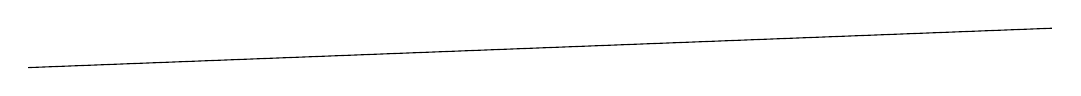
\begin{tikzpicture}\draw (0,0)--(13,.5);\end{tikzpicture}}

% New section, lower half.
\uline{A}

1) Catégorie \inserted{$\mathcal V^\circ$} des Alg. de Poincaré $A$ sur $k$: Alg gr.duées proj. \unsure{de|et} t.f. à degrés $\geq0$; munies d'un hom lin. $\unsure{k|\kappa}_A:A\mathbin{\text{---}}k$ de degré $d^\circ(A)$ dépendant de $A$ tel que $(x,y)\mapsto\unsure{k|\kappa}_A(xy)$ soit une forme \inserted{\uline{strictement}} non dégénérée ---

Les hom\deleted{\unsure{de $\mathcal V^\circ$ sont}}: ce sont les hom d'algèbres gr.duées, sans plus (donc il n'est pas question dans la définition des $\unsure{\mathcal V\mathrm{hom}}$ des $\unsure{k|\kappa}_A$).

\uline{NB} Un isom de cette catégorie n'est pas néc. compatible avec \inserted{les} $\unsure{k|\kappa}_A,\unsure{k|\kappa}_B$.
\margin{\unsure{2|Z}}

2) Foncteur contravariant $\varphi:\unsure{(\mathcal V^{d^\circ=0})|(\mathcal V)^{d^\circ=0}}\longrightarrow\mathrm{Mod\ gr.d}(k)$

\quad a) Sur les objets: $\varphi(A)=A$ où on oublie la multiplication.

\quad b) Sur les morphismes: soit $f^*:B\mathbin{\text{---}}A$, on pose
\[
\varphi(f^*)=f_*:A\longrightarrow B
\]
défini par la condition que
\[
\underbrace{\unsure{k|\kappa}_A(f^*(b)a)}
=\overbrace{\unsure{k|\kappa}_B(bf_*(a))}.
\]
On vérifie $\varphi(g^*f^*)=\varphi(f^*)\varphi(g^*)$, $\varphi(\mathrm{id})=\mathrm{id}$, et formule de proj.
\[
f_*(a)b=f_*(af^*b)
\]
enfin
\[
\deleted{\unsure{k|\kappa}_B(f_*(a))}\qquad
\unsure{k|\kappa}_Bf_*=\unsure{k|\kappa}_A.
\]
\mspage{26}
\scanpage{28}
\mspage{27}
% Reused typed sheet, read after rotation through 180 degrees.
\begin{center}-2.14-\end{center}

is still closed. Therefore, by definition, $x$ is a point of $\mathcal U$.

Therefore, a quasi-projective geometric quotient $X/\mathbb G_m$ exists. But this implies that the action of $\mathbb G_m$ on $X$ is separated. Therefore, by lemma 0.5, the action of $\mathbb G_m$ on $X$ is proper. \uline{QED}

\figure{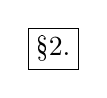
\begin{tikzpicture}[baseline=(heading.base)]\node[draw,inner sep=3pt] (heading) {\S 2.};\end{tikzpicture}} In the last section, we have related the concept of stability with respect to actions of $G$ to the function $\mu^L(x;\lambda)$ involving a 1-parameter subgroup $\lambda$ of $G$. In this section, we shall consider the dependence of $\mu$ on $\lambda$. The analysis leads naturally to an ungainly but remarkable metric space investigated extensively by J. Tits, which we will call the \uline{flag complex} of $G$. The first step is:

\uline{Definition 2.3}/\uline{Proposition 2.6}: Let $G$ be a reductive algebraic group and let $\lambda$ be a 1-PS of $G$. Then there is a unique algebraic subgroup $P(\lambda)\subset G$ such that:
\[
\begin{aligned}
\gamma\in P(\lambda)_k\quad\Longleftrightarrow\quad&
\lambda(\alpha)\cdot\gamma\cdot\lambda(\alpha^{-1})\quad\text{has a specialization in }G\\
&\text{when }\alpha\in(\mathbb G_m)_k\text{ specializes to }0.
\end{aligned}
\]
Moreover, $P(\lambda)$ is a parabolic subgroup of $G$, $\lambda$ is a 1-PS of the radical of $P(\lambda)$, and the specialization $\gamma'$ of $\lambda(\alpha)\cdot\gamma\cdot\lambda(\alpha^{-1})$, as $\alpha\longrightarrow0$, centralizes $\lambda$.

\uline{Proof}: Most of these facts can be seen most easily by means of a faithful representation $\phi:G\longrightarrow\mathrm{GL}(n)$. Recall that the image $\phi(G)$ is \uline{closed} in $\mathrm{GL}(n)$. Therefore, $P(\lambda)=\phi^{-1}(P(\phi\circ\lambda))$, at least as a set of closed points. Now by composing $\phi$ \deleted{$\unsure{\Rightarrow}$}\inserted{with} a suitable inner automorphism of $\mathrm{GL}(n)$, we may assume that $\phi\circ\lambda$ is diagonalized, i.e.
\scanpage{29}
% Top.
Donc on trouve un foncteur \deleted{\unsure{contravariant}}
\[
\mathcal V\longrightarrow\text{Algèbres bivariantes jaugées}.
\]
3) Dans $\mathcal V^\circ$ \deleted{\unsure{il y a}} il y a objet initial: $k$.

Si $A,B\in\mathcal V^\circ$, il existe un coproduit dans $\mathcal V^\circ$ (\unsure{produit} de $\mathcal V$) savoir le produit tensoriel gauche $A\otimes B$. Soit
\[
f^*:A\mathbin{\text{---}}A',\quad g^*:B\mathbin{\text{---}}B',\quad\text{alors}\quad
f^*\otimes g^*:A\otimes B\mathbin{\text{---}}A'\otimes B'
\]
défini par
\[
f^*\otimes g^*(a\otimes b)=f^*(a)\otimes g^*(b)
\]
est l'hom correspondant des coproduits. \deleted{\unsure{On le note}} \inserted{On convient de} mettre sur $A\otimes B$ l'augmentation définie par
\[
\unsure{k|\kappa}_{A\otimes B}=\unsure{k|\kappa}_A\otimes\unsure{k|\kappa}_B
\]
(produit tensoriel \uline{gauche} d'homs homogènes d'\unsure{espaces} gradués).
\margin{i.e.\quad $\unsure{k|\kappa}_{A\otimes B}(x\otimes y)=\unsure{k|\kappa}_A(x)\unsure{k|\kappa}_B(\unsure{x|y})(-1)^{Bx}$}
\margin{produit tensoriel \uline{gauche} d'\unsure{homom.} \uline{homogènes} des \deleted{groupes}\inserted{modules} gr.dués}
\deleted{\unsure{On démontre que}}\quad\inserted{On a alors}
\[
\varphi(f^*\otimes g^*)=\varphi(f^*)\otimes\varphi(g^*)
\]
\margin{\unsure{2|Z}}
i.e.
\[
(*)\qquad(f\times g)_*(a'\otimes b')=f_*(a')\otimes g_*(b')(-1)^{ga'}.
\]
\figure{\begin{tikzpicture}\draw (0,2)--(1,2) .. controls (1.5,2) and (.8,1.5) .. (1.5,1.5)--(5,1.7) .. controls (5.8,1.7) and (5.2,1.2) .. (6,1.3)--(9,1.5);\draw[->] (1.8,.1)..controls (.5,.8) and (1,1.4)..(1.5,1.5);\draw (1.9,-.2)--(1.5,-.2)--(1.5,1.3);\end{tikzpicture}}

% Retraction and replacement signs.
\uline{Mais c'est faux} si on ne suppose pas $f$ et $g$ de degrés pairs.

Les deux mb. de la formule $(*)$ diffèrent par un facteur
\[
(-1)^{ag+bf+Bf}.
\]
Si dans la définition de $\unsure{k|\kappa}_{A\otimes B}$ on n'avait pas mis le \uline{signe} $(-1)^{Bx}$, le signe qui viendrait avec ces \unsure{not.}
\[
(-1)^{a'g+bf}.
\]
Si \inserted{en plus} \unsure{on se dispensait du $\otimes$ du produit|on disposait du $\otimes$ du produit} $f_*\otimes g_*$ au sens \deleted{gauche}\inserted{tordu}, et qu'on \deleted{\unsure{pour}} enlève le \uline{signe} $(-1)^{ga'}$; on trouverait donc un signe
\[
(-1)^{bf}=(-1)^{B'f}.
\]
Si on prenait $\unsure{k|\kappa}$ tordu, $\otimes$ ordinaire, le \uline{signe} serait
\[
(-1)^{bf+(AB+A'B')}.
\]
C'est donc le signe où on prend tout ordinaire
\[
(\unsure{k|\kappa}_{A\otimes B}\inserted{{}=\unsure{k|\kappa}_A\otimes\unsure{k|\kappa}_B}\text{ et }f_*\otimes g_*)
\]
qui est le plus simple. Donc on trouve alors
\[
\boxed{(f\times g)_*=(f_*\overset{\mathrm{ord}}\otimes g_*)
(\mathrm{id}_A\otimes\unsure{[\deleted{(-1)^B}(-1)_{B'}]^{\deg f}})}
\]
\margin{\deleted{\unsure{NB}} Il n'y a aucun signe dès que \textcircled{$f$} est pair.}
\mspage{28}
\scanpage{30}
\mspage{29}
% Reused typed sheet, read after rotation through 180 degrees.
\begin{center}-2.17-\end{center}
\[
\begin{aligned}
\lambda(\alpha)\cdot\gamma\cdot\lambda(\alpha^{-1})
&=\chi(\lambda(\alpha^{-1}))\cdot\gamma\\
&=\alpha^{-\bar\chi(\bar\lambda)}\cdot\gamma
\end{aligned}
\]
for $\gamma\in(\mathbb G_a)_k$. Therefore $\lambda(\alpha)\cdot\gamma\cdot\lambda(\alpha^{-1})$ has a finite specialization when $\alpha\longrightarrow0$, i.e. $\mathbb G_a\subset P(\lambda)$. Therefore $B\subset P(\lambda)$. \uline{QED}

\uline{Proposition 2.7}: Let a reductive group $G$ act via $\sigma$ on a scheme $X$, proper over $k$. Then for all $x\in X_k$, $L\in\mathrm{Pic}^G(X)$, and 1-PS's $\lambda$ of $G$,
\[
\mu^L(x,\lambda)=\mu^L(x,\gamma^{-1}\cdot\lambda\cdot\gamma)
\]
if $\gamma\in P(\lambda)_k$.

\uline{Proof}: Let $y$ be the specialization of $\sigma(\lambda(\alpha),x)$ as $\alpha\longrightarrow0$. Suppose we write $y=\lim_{\alpha\to0}\sigma(\lambda(\alpha),x)$. In this notation, we calculate:
\[
\begin{aligned}
&\lim_{\alpha\to0}\sigma(\gamma^{-1}\cdot\lambda(\alpha)\cdot\gamma,x)\\
&\quad=\lim_{\alpha\to0}\sigma\bigl(\gamma^{-1}\cdot\lambda(\alpha)\cdot\gamma\cdot\lambda(\alpha^{-1}),\sigma(\lambda(\alpha),x)\bigr)\\
&\quad=\sigma\bigl(\gamma^{-1}\cdot\lim_{\alpha\to0}\lambda(\alpha)\cdot\gamma\cdot\lambda(\alpha^{-1}),y\bigr).
\end{aligned}
\]
Let $\lim_{\alpha\to0}\lambda(\alpha)\cdot\gamma\cdot\lambda(\alpha^{-1})=\gamma'$. According to Proposition 2.6, $\gamma'$ centralizes $\lambda$. Now $\mu(x,\gamma^{-1}\cdot\lambda\cdot\gamma)$ is calculated by looking at $\lim_{\alpha\to0}\sigma(\gamma^{-1}\cdot\lambda(\alpha)\cdot\gamma,x)$. Therefore:
\[
\mu(x,\gamma^{-1}\cdot\lambda\cdot\gamma)
=\mu(\sigma(\gamma^{-1}\cdot\gamma',y),\gamma^{-1}\cdot\lambda\cdot\gamma)
\]
By property (i) of $\mu$ (\S1 above), we have:
\scanpage{31}
Pour le reste, on se borne aux $\uline{f}=(\unsure{f^*|g^*},f_*)$ de \uline{degré pair}, donc on trouve $(f\times g)_*=f_*\overset{\mathrm{ord}}\otimes g_*$.

Considérons l'isom de symétrie de $A\otimes B$ vers $B\otimes A$ [considérés comme produits cart. dans $\mathcal V$], on vérifie que c'est $s(x\otimes y)=(-1)^{xy}y\otimes x$. On a bien, comme il convient
\[
\begin{array}{ccc}
(g\times f)_*(\underbrace{s(x\otimes y)}_{y\otimes x\,(-1)^{xy}})
&=&s(\underbrace{(f\times g)_*(x\otimes y)}_{f_*(x)\otimes g_*(y)})\\
\Vert&&\\
g_*(y)\otimes f_*(x)(-1)^{xy}&&g_*(y)\otimes f_*(x)(-1)^{(x+f)(y+g)}
\end{array}
\]

Prouvons les formules de projection
\diagram{\begin{tikzcd}
X\arrow[d,"f"'] & X\times S\arrow[l,"q"']\arrow[d,"f'"]\\
Y\deleted{\unsure{S}} & Y\times S\arrow[l,"\unsure{p}"']
\end{tikzcd}}
\[
\left\{\begin{aligned}
p^*(f_*(x))&=f'_*(q^*(x))\\
f^*(p_*(u))&=q_*(f'^*(u))
\end{aligned}\right.
\]
\diagram{\begin{tikzcd}
x\in B\arrow[r,"q^*(b)=b\otimes1"] & B\otimes\unsure{R}\,\\
A\arrow[u,"f^*"]\arrow[r,"p^*(a)=a\otimes1"'] & A\otimes R\arrow[u,"f^*\otimes\mathrm{id}_R=\unsure{f'_*|f'^*}"']
\end{tikzcd}}
\[
f_*(x)\otimes1=(f_*\otimes1)(x\otimes1)\qquad\mathrm{OK}
\]
\[
\begin{array}{ccc}
f^*\bigl(\underbrace{(\mathrm{id}_A\otimes\unsure{k|\kappa}_R)(a\otimes r)}_{\deleted{\unsure{a\otimes k(r)}}\,\inserted{k(r)a}}\bigr)
&\overset{?}=&(\mathrm{id}_B\otimes\unsure{k|\kappa}_R)\underbrace{(f^*\otimes\mathrm{id}_R)(a\otimes r)}_{\unsure{f'(a)r|f^*(a)r}}\\
\Vert&&\\
\unsure{k|\kappa}(r)f^*(a)&&\unsure{k|\kappa}(r)f^*(a)\quad\mathrm{O.K.}
\end{array}
\]
\figure{\begin{tikzpicture}\draw (0,.5)--(4,.8)..controls(4.8,.9)and(4.4,0)..(5.2,0)--(12.5,.2);\end{tikzpicture}}

\diagram{\begin{tikzcd}
X\arrow[r,"f"]&Y\arrow[r,dash,"g"]&Z
\end{tikzcd}\qquad\begin{tikzcd}
A&B\arrow[l,"f^*"']&C\arrow[l,"g^*"']
\end{tikzcd}}
\diagram{\begin{tikzcd}[column sep=large]
&X\arrow[dl,"\Gamma_{gf}"']\arrow[dr,"\Gamma_f"]&\\
X\times Z\arrow[dr,"\Gamma_f\times\mathrm{id}_Z=\lambda"']&&X\times Y\arrow[dl,"\mathrm{id}_X\times\Gamma_g=\lambda'"]\\
&X\times Y\times Z&
\end{tikzcd}}
\diagram{\begin{tikzcd}[column sep=large]
&\begin{gathered}af^*(b)\cdot f^*(g^*(c))\\A\end{gathered}&\\
A\otimes C\arrow[ur]&&A\otimes B\arrow[ul]\\
(af^*(b))\otimes c& A\otimes B\otimes C\arrow[ul,"\lambda^*"]\arrow[ur,"\lambda'^*"']&a\otimes bg^*(c)\\
\deleted{\unsure{a\otimes b}}\arrow[u]&a\otimes b\otimes c&
\end{tikzcd}}
\[
\lambda'^*(\lambda_*(u))=(\Gamma_f)_*(\Gamma_{gf}^*(u))
\]
et formule symétrique.

\margin{\uline{Question} Trouver un cas général commun où la formule d'échange est valable. Suffit-il que le produit fibré existe dans $\mathcal V$ et que les dim. soient correctes?}
\figure{\begin{tikzpicture}\draw(0,0)--(0,2)..controls(0,2.2)and(.2,2.3)..(.5,2.35)--(5,3.3);\end{tikzpicture}}
\mspage{30}
\scanpage{32}
\mspage{31}
% Reused typed sheet, read after rotation through 180 degrees.
\begin{center}-2.13-\end{center}
\[
\phi=\psi_1\cdot\langle\lambda\rangle\cdot\psi_2
\]
for $R$-valued points $\psi_1$ and $\psi_2$ of $G$, and some 1-PS $\lambda$. Moreover $\lambda$ is non-trivial since $\phi$ is not an $R$-valued point of $G$. But then
\[
\xi'=\sigma(\psi_2,\xi)
\]
and
\[
\sigma(\langle\lambda\rangle,\xi')=\sigma(\psi_1^{-1},\sigma(\phi,\xi))
\]
are both $R$-valued points of $X$. In other words, the $K$-valued, but not $R$-valued point $\langle\lambda\rangle\times\xi'$ of $G\times X$ is mapped by $\unsure{\Psi|\bar\Psi}$ to an $R$-valued point of $X\times X$. Since by definition, $\langle\lambda\rangle$ is induced from a $K$-valued point of $\mathbb G_m$ via $\lambda:\mathbb G_m\longrightarrow G$, this means that the composite morphism $\unsure{\Psi|\bar\Psi}\circ(\lambda\times1_X):\mathbb G_m\times X\longrightarrow X\times X$ is not proper, i.e. the induced action of $\mathbb G_m$ is not proper. \uline{QED}

\uline{Corollary 2.5}: Let a reductive algebraic group $G$ act on an algebraic pre-scheme $X$. Let $L\in\mathrm{Pic}^G(X)$. Then $G$ acts properly on $X^s_{(0)}(L)$.

\uline{Proof}: Without loss of generality, we may replace $X$ by $X^s_{(0)}(L)$: then $L$ is ample on $X$, and $X$ is a scheme. By the above proposition, it suffices to prove that for every non-trivial 1-PS $\lambda$ of $G$, the induced action of $\mathbb G_m$ is proper. Fix some $\lambda$. Let $\mathcal U$ be the open set in $X$ of points properly stable for the induced action of $\mathbb G_m$: then I claim $\mathcal U=X$. For if $x$ is a geometric point of $X$, then $x$ has an affine neighborhood $X_s$, where $s$ is an invariant section of $L^N$, and such that all stabilizers of points of $X_s$ are 0-dimensional. But then $s$ is invariant under $\mathbb G_m$, and the action of $\mathbb G_m$ on $X_s$
\scanpage{34}
\uline{Catégorie des algèbres bivariantes} (sur un anneau $k$)

C'est la catégorie dont les objets sont les $k$-algèbres \inserted{\uline{muni d'une forme} $\unsure{k|\kappa}_A:A\mathbin{\text{---}}k$}, et les morphismes de $A$ dans $B$ les couples $f=(f_*,f^*)$, où $f^*:B\mathbin{\text{---}}A$ est un hom d'algèbres, et où $f_*:A\mathbin{\text{---}}B$ est un hom $B$ linéaire \inserted{(à g. et à dr.)}, i.e. un hom additif satisfaisant les ``form. de projection''
\[
(*)\qquad[f_*(xf^*(y))=f_*(x)y],\quad f_*(f^*(y)x)=yf_*(x).
\]
\margin{(signe $(-1)^{\delta j}$ \unsure{raisonnable} ds le cas gradué; si la deux. formule est valable, $y$ de degré $j$, $f_*$ de degré $\delta$.)}
\margin{Il faut choisir entre l'une et l'autre formule!}
et de plus:
\[
(**)\qquad\unsure{k|\kappa}_Bf_*=\unsure{k|\kappa}_A.
\]
On a une variante gr.duée, \deleted{et} On aura à travailler dans diverses sous-catégories pleines, ou même non pleines.

Dans le cas gradué anticommutatif (où $f^*$ est donc un hom d'Alg. gr.duées, et \unsure{où} $f_*$ préserve à translation \inserted{\uline{de degré pair}} près la graduation), les deux formules $(*)$ sont équivalentes.

\margin{\uline{Remarque} \unsure{Bien que|Pour que} $(f_*,f^*)$ soit un isomorphisme, \unsure{il faut que $f^*$ et} \deleted{\unsure{un isom de}} $f_*$ \unsure{bijectifs}, i.e. $f^*$ un isom et $f_*(1)$ inversible; les ``bons'' isom. sont ceux où $f_*(1)=1$, ou encore $f_*$ et $f^*$ inverses l'un de l'autre.}
\figure{\begin{tikzpicture}\draw(0,5)..controls(1,6)and(1.7,5.8)..(1.8,4.5)..controls(1.8,4)and(2.3,4.3)..(2.7,4)..controls(3,3.7)and(2.5,3.6)..(2.5,3.1)--(2.4,1.2)..controls(2.2,.6)and(1.5,.3)..(.3,0);\end{tikzpicture}}

Soit $A$ une algèbre muni d'une forme
\[
\unsure{k|\kappa}_A:A\mathbin{\text{---}}k
\]
\deleted{que}\inserted{donc} la forme bilinéaire
\[
(x,y)\mapsto\unsure{k|\kappa}(xy)
\]
sur $A\times A$ \deleted{est séparée, donc} définit un hom. \inserted{\unsure{(= dual!)}} \deleted{injectif}
\[
\varphi_A:A\longrightarrow\check A\qquad(\check A:\mathrm{Hom}_{k\text{-}\mathrm{mod}}(A,k)).
\]
\inserted{$\langle y,\varphi_A(x)\rangle=\unsure{k|\kappa}(yx)$}
\margin{\deleted{\unsure{l'isomorphisme $\mathcal V(B)\mathbin{\text{---}}\mathcal V(A)$}}}
Supposons que $B$ est de même muni de $\unsure{k|\kappa}_B:B\mathbin{\text{---}}k$, \inserted{et que $\varphi_B$ soit \uline{injectif}}, et soit $f^*:B\longrightarrow A$ tel que l'hom transposé ${}^tf^*:\check A\mathbin{\text{---}}\check B$ \unsure{applique|vérifie} $\mathrm{Im}\,\varphi_A$ dans $\mathrm{Im}\,\varphi_B$ [ce qui n'est pas une restriction si $\varphi_B:B\overset{\sim}\longrightarrow\check B$!].

Alors l'application induite, \inserted{notée} $f_*$, est donc caractérisée par
\[
(***)\qquad\unsure{k|\kappa}(yf_*(x))=\unsure{k|\kappa}(f^*(y)x)
\]
et satisfait de ce fait la $2^{\text{ième}}$ relation $(*)$, [donc la première dans le cas commutatif, ou gradué anticommutatif, quand $f_*$ est hom à translation \inserted{paire} près].
\inserted{De plus, il satisfait $(**)$ (faire $y=1$ dans $(***)$).}
\deleted{\unsure{Supposons donc $A,B$}}

% Addition on the lowest edge of the sheet.
\inserted{Réciproquement \unsure{étant donné un hom} $(f^*,f_*)$ de $(A,\unsure{k|\kappa}_A)$ dans $(B,\unsure{k|\kappa}_B)$, $f_*$ satisfait $(***)$ ce qui \unsure{le} détermine par $f^*$. \deleted{\unsure{$\unsure{k|\kappa}_A$ dans $\unsure{k|\kappa}_B$, de $(**)$ donc $f_*$ est}}}
\mspage{33}
\scanpage{35}
\mspage{34}
% Reused typed sheet, read after rotation through 180 degrees.
\begin{center}-3.11-\end{center}
Moreover, the section:
\[
(D_{\alpha_0,\ldots\alpha_n})^{n+1}\in\Gamma(\mathcal U_{\mathrm{reg}},L_{\alpha_0}^{n+1}\otimes\cdots\otimes L_{\alpha_n}^{n+1})
\]
is invariant in the $\mathrm{SL}(n+1)$-linearization of this sheaf, hence in the $\mathrm{PGL}(n)$-linearization of this sheaf, . Therefore, according to SGA 8, \S1, there is a section $E_{\alpha_0,\ldots\alpha_n}$ of $M_{\alpha_0}\otimes\cdots\otimes M_{\alpha_n}$ such that:
\[
(D_{\alpha_0,\ldots\alpha_n})^{n+1}=\unsure{\Phi|\bar\Phi}^{*}(E_{\alpha_0,\ldots\alpha_n}).
\]
\figure{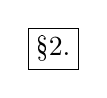
\begin{tikzpicture}[baseline=(heading.base)]\node[draw,inner sep=3pt] (heading) {\S2.};\end{tikzpicture}} The purpose of this section is to show that although $M_0\otimes\cdots\otimes M_m$ is not ample on $Z$ - which is not even a scheme - it is ample on a fairly large open subset $Z_0\subset Z$. We first define the subset $\unsure{\Phi|\bar\Phi}^{-1}(Z_0)$ of $\mathcal U_{\mathrm{reg}}$:

\uline{Definition 3.7}/\uline{Proposition 3.4}: $\mathcal U_{\mathrm{stable}}$ is the open subset of $(\mathbb P_n)^{m+1}$ whose geometric points $x=(x^{(0)},\ldots,x^{(m)})$ are those points such that for every proper linear subspace $L\subset\overline{\mathbb P}_n$:
\[
\frac{\text{number of points }x^{(i)}\text{ in }L}{m+1}<\frac{\dim L+1}{n+1}.
\]
\uline{Proof}: Consider the set of all pairs $\{I,n_0\}$ consisting of a subset $I\subset\{0,1,\ldots,m\}$ and an integer $n_0$ between 0 and $n-1$ such that:
\[
\frac{\text{cardinality of }I}{m+1}\geq\frac{n_0+1}{n+1}.
\]
Then the set of geometric points \uline{not} satisfying the above condition is the (finite) union over all $\{I,n_0\}$ of the sets consisting of
\scanpage{36}
% Continuation.
gr.duées anticommutatives, $f^*$ homogène. Supposons qu'il existe un entier $d=d(A)$ tel que $\unsure{k|\kappa}_A$ soit composé
\diagram{\begin{tikzcd}
A\arrow[r,dash]&A^d\arrow[r,"\unsure{k|\kappa}_A^{(d)}"]&k
\end{tikzcd}}
et de même un $d'=d(B)$. Alors si $x$ est de degré $i$, la forme $\varphi_A(x)$ est nulle en degré $\ne d-i$, donc
\[
\langle f^*(y),\varphi_A(x)\rangle=\unsure{k|\kappa}(f^*(y)x)
\]
est nul en degré $\ne\unsure{d-i'|d-i}$;
\deleted{donc si $f$} de $=$, \inserted{si $x'$ \deleted{$\unsure{{}=f_*(x)}$} est hom de degré $i'$}, la forme $\varphi_B(x')$ est nulle en degré $\ne d'-i'$, donc on doit avoir (si $f_*(x)\ne0$)
\[
d-i=d'-i'\qquad\text{i.e.}\qquad i'=i+(d'-d).
\]
Si alors on pose $f_*(x)=\sum_jx'_j$, on voit que l'effet de la forme $\varphi_A(f_*(x))$ sur $B^{d'-j}$ est égal à $\varphi_B(x'_j)$, donc est nul si $\deleted{j}\inserted{d'-j}\ne d-i$, donc dans ce cas $x'_j=0$. Donc $f_*$ \uline{augmente les degrés de} $\unsure{d'-d|d'+d}$.

Nous travaillons dans la catégorie \inserted{bivariante} des Algèbres graduées anticommutatives, munies d'un degré $d$, le $f_*:A\longrightarrow B$ étant assujetti à être de degré $d(B)-d(A)$, \inserted{et $\unsure{k|\kappa}_A$ devant factoriser par $A^{d(A)}$}. La sous catégorie pleine des $A$ tels que $d(A)$ pair est commode [et il y a lieu parfois de se borner aux Algèbres $A$ qui sont à degrés \deleted{dans}\inserted{dans} $[0,d(A)]$]. Il n'est pas \deleted{utile}\inserted{commode} de se borner aux ``algèbres de Poincaré'', \unsure{associée|associées} comme dessus à une forme sur $A$, car les constructions universelles qu'on va faire en feront de tte façon sortir!
\mspage{35}
\scanpage{37}
\mspage{36}
% Reused typed sheet, read after rotation through 180 degrees.
\begin{center}-3.9-\end{center}
leaves $x$ fixed. Secondly, $3)\Rightarrow1)$ is an immediate consequence of Proposition 2.1.

Thirdly, we will prove that $2)\Rightarrow3)$. By virtue of 2), all the points $x_i$ cannot lie in one hyperplane, hence we can choose $n+1$ of the $x_i$ which are not in one hyperplane, say $x^{(0)},x^{(1)},\ldots,x^{(n)}$. Without loss of generality, we may assume that $x^{(i)}$ has homogeneous coordinates $x_j^{(i)}=\delta_{ij}$. Now for each $n+k$ between $n+1$ and $m$, let $S'_k$ be the set of integers $i$ such that
\[
D_{0,1,\ldots,\hat i,\ldots,n,n+k}\ne0,
\]
i.e. $x^{(n+k)}$ is not in the hyperplane spanned by $x^{(0)},\ldots,\widehat{x^{(i)}},\ldots,x^{(n)}$. Then I claim that there is no partition of the set $\{0,1,\ldots,n\}$ into 2 disjoint subsets $T'$ and $T''$ such that every $S'_k$ is contained in $T'$ or $T''$. For if there were, and if one let $L'$ (resp.$L''$) be the linear subspace defined by $X_i=0$ for all $i\in T'$ (resp. $i\in T''$), then every point $x^{(k)}$ would be in $L'\cup L''$. It follows immediately that a suitable set of subsets $S_i\subset S'_i$ is an R-partition $R$ and that $x\in\mathcal U_R$. \uline{QED}

From this Proposition, it is clear that $\mathcal U_{\mathrm{reg}}$ is precisely the set of pre-stable points of $(\mathbb P_n)^{m+1}$, in the sense of Chapter 1.

Our next step is to construct a geometric quotient of $\mathcal U_{\mathrm{reg}}$ by $\mathrm{PGL}(n)$: let $\mathcal U_1,\ldots,\mathcal U_N$ be the open subsets $\mathcal U_R$ of $\mathcal U_{\mathrm{reg}}$ and the subsets obtained from these by permuting the coordinates. Let $(Z_i,\phi_i)$ be the geometric quotient of $\mathcal U_i$ by $\mathrm{PGL}(n)$. For all pairs $i,j$, $\mathcal U_i\cap\mathcal U_j$ is an invariant open subset in $\mathcal U_i$ and in $\mathcal U_j$.
\scanpage{38}
\mspage{37}
% Top: cancelled opening and tensor product.
\deleted{Soient $A$ et $B$ deux algèbres}

Le produit tensoriel gradué gauche $A\otimes B$ est un foncteur sur la catégorie $C$ \inserted{bivariante} des algèbres graduées. Ce produit tensoriel (malheureusement!) ne s'interprète pas comme un produit dans la catégorie bivariante: car on n'a pas d'hom de $C$ \unsure{canonique} $f:A\longrightarrow A\otimes A$, $f=(f^*,f_*)$, qui jouerait le rôle d'une application diagonale. On trouve néanmoins que c'est un produit \inserted{dans $C$} quand $A,B$ sont toutes deux des Alg. de Poincaré\ldots

% Middle: simplicial object and special condition.
Algèbre bivariante simpliciale: c'est un objet simplicial (pas \uline{$\frac12$} simplicial!) de la catégorie des Algèbres bivariantes, donc un foncteur contravariant de la catégor. des ens finis non vides dans $C$. Il est ``\uline{spécial}'' s'il transforme sommes disjointes en ``produits tensoriel'', i.e. si pour $I=I'\amalg I''$, les hom
\[
A(I')\xrightarrow{\alpha^*} A(I),\quad A(I'')\xrightarrow{\beta^*} A(I)
\]
[où $\alpha:I'\longrightarrow I$, $\beta:I''\longrightarrow I$) définissent un \uline{isom}
\[
A(I')\otimes A(I'')\xrightarrow{\sim}A(I'\amalg I'').
\]

% Bottom: Poincare restriction.
Si \deleted{$A(\Delta^0)$ est une Algèbre} on se borne à la sous-catégorie pleine des Alg. biv. simpliciales $A(\unsure{\bullet|\sigma})$ telles que $A(\unsure{\Delta^0})=A_0$ soit une Algèbre de Poincaré, on trouve une \uline{équivalence} de la catégorie des Alg. biv. simpliciales et des alg. de Poincaré.
\scanpage{39}
\mspage{38}
% Reused typescript, upside down relative to the handwritten foliation.
\begin{center}-3.8-\end{center}
Our next aim is to show that we have enough open sets:

\uline{Definition 3.6}: For fixed $m$, let $\mathcal U_{\mathrm{reg}}$ be the union of all the open subsets $\mathcal U_R$ and their images under permutations of the factors of $(\mathbb{P}_n)^{m+1}$.

\uline{Proposition 3.3}: Let $x=(x^{(0)},x^{(0)},\ldots,x^{(m)})$ be a geometric point of $(\mathbb{P}_n)^{m+1}$. Then the following are equivalent:

(1) the stabilizer $S(x)$ is $0$ dimensional,

(2) there do not exist disjoint proper linear subspaces $L'$ and $L''$ in $\overline{\mathbb{P}}_n$ such that every $x^{(i)}$ is in either $L'$ or $L''$,

(3) $x$ is a geometric point of $\mathcal U_{\mathrm{reg}}$.

\uline{Proof}: Let $k$ be the algebraically closed field over which $x$ is defined. For simplicity, we shall write $\mathbb{P}_n$ for $\mathbb{P}_n\times k$, $\mathcal U_R$ for $\mathcal U_R\times k$, etc. in the course of this proof. First, the implication $1)\Rightarrow 2)$ is clear: for, in suitable homogeneous coordinates $\{x_i\}$, one may assume that:
\[
\begin{aligned}
L'&\subset\{x_0=x_1=\ldots=x_r=0\}\\
L''&\subset\{x_{r+1}=\ldots=x_n=0\}.
\end{aligned}
\]
Then the subgroup of transformations:
\diagram{\begin{tikzcd}[row sep=1.3em,column sep=1.2em,execute at end picture={
\draw ([xshift=-6pt,yshift=6pt]\tikzcdmatrixname-1-1.north west) -- ++(-5pt,0) |- ([xshift=-6pt,yshift=-6pt]\tikzcdmatrixname-4-1.south west);
\draw ([xshift=6pt,yshift=6pt]\tikzcdmatrixname-1-4.north east) -- ++(5pt,0) |- ([xshift=6pt,yshift=-6pt]\tikzcdmatrixname-4-4.south east);
\draw[dashed] ([xshift=-5pt]\tikzcdmatrixname-2-1.south west) -- ([xshift=5pt]\tikzcdmatrixname-2-4.south east);
\draw[dashed] ([xshift=7pt,yshift=5pt]\tikzcdmatrixname-1-2.north east) -- ([xshift=7pt,yshift=-5pt]\tikzcdmatrixname-4-2.south east);
\draw ([xshift=-1.4cm,yshift=4pt]\tikzcdmatrixname-1-1.north west) -- ++(0.4cm,0);
\draw ([xshift=-1.4cm]\tikzcdmatrixname-2-1.south west) -- ++(0.4cm,0);
\draw ([xshift=-1.4cm,yshift=-4pt]\tikzcdmatrixname-4-1.south west) -- ++(0.4cm,0);
\draw[<->] ([xshift=-1.2cm]\tikzcdmatrixname-1-1.north west) -- node[fill=white] {$r+1$} ([xshift=-1.2cm,yshift=4pt]\tikzcdmatrixname-2-1.south west);
\draw[<->] ([xshift=-1.2cm,yshift=-4pt]\tikzcdmatrixname-2-1.south west) -- node[fill=white] {$n-r$} ([xshift=-1.2cm]\tikzcdmatrixname-4-1.south west);
}]
\alpha\arrow[dr,dashed,no head] & 0 & \vphantom{0} & \vphantom{0}\\
0 & \alpha & \vphantom{0} & 0\\
\vphantom{0}&0&\beta\arrow[dr,dashed,no head]&0\\
\vphantom{0}&\vphantom{0}&0&\beta
\end{tikzcd}}
\scanpage{40}
\mspage{39}
% Top proposition and three conditions, with inserted c).
\uline{Proposition} Pour tout $n\geq1$, soit $A_n\subset H^*(X^n)$ un \unsure{ss-vectoriel} \uline{stable} \inserted{par \uline{grp sym.}}.
Conditions équivalentes:

\unsure{(i)} a) Pour tout \deleted{$u\in H^*$} $u\in A_{n+m}\subset H^*(X^n\times X^m)$ et $x\in A_n\in H^*(X^n)$, on a $u(x)\in H^*(X^m)$.

b) Si $x\in A_n$, $y\in A_m$, alors $x\otimes y\in A_{n+m}$; pour tt $n$, $1\in A_n$.

\inserted{c) Pour \unsure{tte|toute} surjection $[1,n+1]\longrightarrow[1,n]$, son graphe dans $H^*(X^n\times X^{n+1})\in A_{2n+1}$. \unsure{Et $=$ chose pour tte injection|Et de même pour tte injection} $[1,n]\unsure{\lhook\joinrel\relbar|\subset}[1,n+1]$}

\unsure{(ii)} Les \deleted{\unsure{systèmes de}} $A_n$ sont des \uline{sous-algèbres}, stables par images inverses \inserted{et images directes} par \uline{projections} $X^{n+1}\longrightarrow X^n$, et \deleted{par images inverses} par images directes par injections $X^n\unsure{\lhook\joinrel\relbar|\hookrightarrow}X^{n+1}$.

\figure{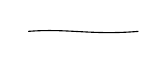
\begin{tikzpicture}\draw (0,0) .. controls (.5,.04) and (.8,-.05) .. (1.4,0);\end{tikzpicture}}

Ces conditions impliquent que les $A_n$ sont stables par ttes images inv. et images dir. par tte application simpliciale \inserted{$X^n\longrightarrow X^m$}, et que \deleted{\unsure{$A_n$}} pour tte telle application, $H^*(X^n\times X^m)$ \unsure{cont.} la classe du graphe\ldots

% Lower paragraph.
(iii) \unsure{Considérons} $A_{n+m}\in H^*(X^n\times X^m)$ comme un ens d'hom de $H^*(X^n)$ en $H^*(X^m)$, on veut que ces ens. soient stables par composition $(n,m\geq0)$, contiennent les identités, soient stables par $\unsure{\boxtimes|\otimes}$, et contiennent les hom images inverses et directes par une application simpliciale.
\scanpage{41}
\mspage{40}
% Reused typescript, upside down relative to the foliation.
\begin{center}-3.13-\end{center}
The key property of stable geometric points turns out to be the following:

\uline{Proposition 3.6}: Let $x$ be a geometric point of $(\mathbb{P}_n)^{m+1}$. Then $x$ is stable if andonly if there are integers $N\geq N_0>0$ and there are monomials $P_0,\ldots,P_m$ in the expressions $D_{\alpha_0,\ldots,\alpha_n}$ such that, for $0\leq i\leq m$:

(i) $P_i$ is a section of $L_0^N\otimes\cdots\otimes L_i^{N-N_0}\otimes\cdots\otimes L_m^N$

(ii) $P_i(x)\ne0$

\uline{Proof}: Let $E=(\mathbb{R})^{m+1}$ be Euclidean space of dimension $m+1$. To each $D_{\alpha_0,\ldots,\alpha_n}$ associate a point $d_{\alpha_0,\ldots,\alpha_n}\in E$ as follows:
\[
\begin{aligned}
d_{\alpha_0,\ldots,\alpha_n}&=(\epsilon_0,\epsilon_1,\ldots,\epsilon_m)\\
\epsilon_i&=0\text{ if }i\notin\{\alpha_0,\ldots,\alpha_n\}\\
\epsilon_i&=1\text{ if }i\in\{\alpha_0,\ldots,\alpha_n\}
\end{aligned}
\]
Then $d$ determines which invertible sheaf $D$ is a section of. More generally, to any monomial $P$ is the $D$'s, \unsure{associate the corresponding|associatethe corresponding} sum of the $d$'s. Now define $C_x$ to be the convex cone spanned by those points $d_{\alpha_0,\ldots,\alpha_n}$ such that $D_{\alpha_0,\ldots,\alpha_n}(x)\ne0$, i.e. such that the components $x^{(\alpha_0)},\ldots,x^{(\alpha_n)}$ do not lie in a hyperplane. Then it is easy to see that:
\scanpage{42}
\mspage{41}
% Top definitions; a note points to the bracketed adjective.
Catégorie des $k$-algèbres [\uline{graduées}] bivariantes \inserted{anticommutatives} (munies d'un degré $d(A)$, nulles en degré $\notin[1,d(A)]$; on ne donne pas de $\unsure{k_A|\kappa_A}:A\mathbin{-}k$).
\margin{\unsure{les hom sont homogènes.}}

Objet particulier de cette catégorie: $k$ de degré $0$.

Algèbre graduée bivariante \uline{jaugée}: muni d'un hom dans $k$.
Dans certains cas d'hom de telles, $f_*$ est déterminé par $f^*$. $(*)$

Produit tensoriel d'Algèbres bivariantes (resp. jaugées). Dans certains cas, c'est un produit dans la catégorie des Algèbres bivariantes jaugées.

% Middle: simplicial special case.
Algèbre graduée bivariante \inserted{(resp. gr. biv. jaugée)} \uline{simpliciale}. \deleted{\unsure{resp.}} Cas \uline{spécial}: on a
\[
A(I'\amalg I'')\xleftarrow[\sim]{(\alpha^*,\beta^*)}A(I')\otimes A(I''),
\]
d'autre part si $\alpha:I\mathbin{-}J$, $\beta:I'\longrightarrow J'$, sur $\alpha\amalg\beta=\gamma:I\amalg I'\mathbin{-}J\amalg J'$, on veut que $(\alpha\amalg\beta)_*:A(\unsure{J\amalg J'})\mathbin{-}A(I\amalg I')$ s'identifie à $\alpha_*\otimes\beta_*$. On voit que si $A(\Delta^0)=A_0$ est ``de Poincaré'' (cas jaugé) $A(\unsure{\bullet})\mathbin{-}A(\unsure{\varnothing|\omega})$ est \unsure{une jauge}, alors $A(\unsure{\bullet})$ est \unsure{Alg.} de Poincaré, et des alg. de Poincaré.

Et $A(\unsure{\bullet})\unsure{\mathbin{-}|\longmapsto}(A_0,\delta)$ est un foncteur pl. fidèle de la catégorie des Alg. graduées bivariantes jaugées simpliciales, dans la catégorie des algèbres \inserted{gr.} bivariantes jaugées $A$, munies d'un $\Delta\in[A\otimes A]^{d(A)}_{\unsure{0}}$ [il convient de préciser les axiomes à mettre sur ce $\Delta$]
\margin{\uline{à vérifier}; il faut d'abord voir qu'il suffit de connaître $\delta_*:A\longrightarrow A\otimes A$; \unsure{en posant} $\Delta=\delta_*(1)$}

% Example, with revisions and left marginal coefficient-field qualification.
\uuline{Ex} 1) Si on a une théorie ch. \deleted{\unsure{sur les variétés}} [satisfaisant Künneth et Poincaré)] sur la catégorie \inserted{$\unsure{\mathcal V|V}$} des variétés complètes algébriques non \uline{singulières} de dim $d$, \deleted{\unsure{sur un corps}} \inserted{sur un corps donné}, d'où un foncteur \inserted{cov} de $\unsure{\mathcal V|V}$ dans la catégorie $C_{\mathrm{jaug}}$ des Alg. gr. bivar. \uline{jaugées} sur $k$, et en \unsure{transformant} par ce foncteur l'objet simplicial canonique $I\longmapsto X^I$ défini par $X\in\unsure{\mathcal V|V}$, on trouve une Algèbre bivariante simpliciale bivariante jaugée canonique, d'ailleurs définie axiomatiquement, comme dit plus haut, par \unsure{sa composante} $H^*(X)$\ldots
\margin{$k$ un \uline{corps}}

\figure{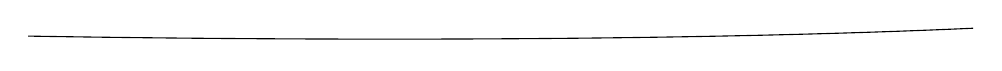
\begin{tikzpicture}\draw (0,0) .. controls (3,-.05) and (8,-.08) .. (12,.1);\end{tikzpicture}}
% Footnote corresponding to (*).
$(*)$ Attention, les \uline{isom} $(f^*,f_*)$ ne sont pas néc. tels que $f_*=f^{*-1}$ i.e. $f_*(1)=1$ ($\Rightarrow$ \deleted{\unsure{pas}} que $k_Af^*=k_B$), ex: $f^*=\mathrm{id}$, $f_*(y)=y\sigma$ $(\sigma\in A^*)$, $k_B(y)=k_A(y\sigma^{-1})$\ldots
